%
% - - - Allgemeine Parameter - - - 
%
% - - - Abgabedatum der Arbeit - - - 
\newcommand{\dateOfSubmission}{1. August 2018}
% - - - Autor - - - 
\newcommand{\authorOfWork}{Martin Leonard Haufs}
% - - - Matrikelnummer - - -
\newcommand{\matrikelnummer}{4015814}
% - - - Studiengang
\newcommand{\studiengang}{Scientific Programming}
% - - - Dokumententyp - - -
\newcommand{\documentTypeName}{Bachelorarbeit}
% - - - Titel der Arbeit
\newcommand{\documenttitle}{Multimediale Unterstützung in der Medizinprodukteaufbereitung mittels Smartglasses}
%
\newcommand{\erstpruefer}{Prof. Dr. Volker Sander}
%
\newcommand{\zweitpruefer}{Dr. Mirco Vitr}
% - - - Dokumentenklasse - - - 
\documentclass[ngerman]{scrreprt}
%
% - - - Header - - - 
%

% 1.5-facher Zeilenabstand:
\usepackage[onehalfspacing]{setspace} 

\usepackage[utf8]{inputenc}
\usepackage[ngerman]{babel}
% Durchgehende Nummerierung von Abbildungen über
% Chapter hinaus
%\usepackage{chngcntr}
%\counterwithout{figure}{chapter}
%
% Kommentare mit \comment{}-Umgebung
\usepackage{verbatim}
%
\usepackage[%
    backend=biber,
    style=numeric,
    %style=alphabetic,
    %citestyle=alphabetic-verb,
    %citestyle=numeric
    %sorting=ynt    % Sortierung nach Name des Autors
    sorting=none    % Sortierung nach Auftreten
]{biblatex}
%\addbibresource{data/bibliography.bib}
\addbibresource{Bachelorarbeit.bib}

\usepackage{fancyvrb}
\usepackage{listings}

\lstset{literate=%
  {Ö}{{\"O}}1
  {Ä}{{\"A}}1
  {Ü}{{\"U}}1
  {ß}{{\ss}}2
  {ü}{{\"u}}1
  {ä}{{\"a}}1
  {ö}{{\"o}}1
}


\usepackage{minted}
\usepackage[german]{fancyref}
\usepackage{enumitem}
\usepackage{array}
\usepackage{graphicx}
\usepackage{multicol}
%\usepackage{pgf-umlsd}
%\usepackage[pict2e]{struktex}
\usepackage{tikz}
%\usetikzlibrary{arrows,shadows}
%\usepackage{csvsimple}
%\usepackage{pgfplots}
\usepackage{filecontents}
%\usepackage{../daten/tikz-uml}

% Anführungsstriche mit \enquote{}-Umgebung
\usepackage[autostyle]{csquotes} 

% =============================
\usepackage[colorinlistoftodos,prependcaption,textsize=tiny]{todonotes}

% Hyperlinks in PDF-Version des Dokumentes. Option sagt, dass keine roten Boxen erzeugt werden sollen.
\usepackage[pdfborder={0 0 0}]{hyperref} 

% Todo commands
% https://mirror.hmc.edu/ctan/macros/latex/contrib/todonotes/todonotes.pdf
\newcommand{\insertMore}[1]{\todo[inline, color=green!40]{#1 ergänzen}}
\newcommand{\insertRef}[1]{\todo[color=blue!40]{#1 (Referenz fehlt)}}
\newcommand{\importantTodo}[1]{\todo[color=red!40]{#1 (Wichtig!)}}

% Programmcode


\begin{comment}

\usepackage{geometry}
\geometry{
  left=2.5cm,
  right=2.5cm,
  top=2cm,
  bottom=2cm,
  bindingoffset=5mm
}

\end{comment}

\definecolor{lightgray}{rgb}{0.95, 0.95, 0.95}
\definecolor{darkgray}{rgb}{0.4, 0.4, 0.4}
%\definecolor{purple}{rgb}{0.65, 0.12, 0.82}
\definecolor{editorGray}{rgb}{0.95, 0.95, 0.95}
\definecolor{editorOcher}{rgb}{1, 0.5, 0} % #FF7F00 -> rgb(239, 169, 0)
\definecolor{editorGreen}{rgb}{0, 0.5, 0} % #007C00 -> rgb(0, 124, 0)
\definecolor{orange}{rgb}{1,0.45,0.13}		
\definecolor{olive}{rgb}{0.17,0.59,0.20}
\definecolor{brown}{rgb}{0.69,0.31,0.31}
\definecolor{purple}{rgb}{0.38,0.18,0.81}
\definecolor{lightblue}{rgb}{0.1,0.57,0.7}
\definecolor{lightred}{rgb}{1,0.4,0.5}
\usepackage{upquote}
% CSS
\lstdefinelanguage{CSS}{
  keywords={color,background-image:,margin,padding,font,weight,display,position,top,left,right,bottom,list,style,border,size,white,space,min,width, transition:, transform:, transition-property, transition-duration, transition-timing-function},	
  sensitive=true,
  morecomment=[l]{//},
  morecomment=[s]{/*}{*/},
  morestring=[b]',
  morestring=[b]",
  alsoletter={:},
  alsodigit={-}
}

% JavaScript
\lstdefinelanguage{JavaScript}{
  morekeywords={typeof, new, true, false, catch, function, return, null, catch, switch, var, if, in, while, do, else, case, break},
  morecomment=[s]{/*}{*/},
  morecomment=[l]//,
  morestring=[b]",
  morestring=[b]'
}

\lstdefinelanguage{HTML5}{
  language=html,
  sensitive=true,	
  alsoletter={<>=-},	
  morecomment=[s]{<!-}{-->},
  tag=[s],
  otherkeywords={
  % General
  >,
  % Standard tags
	<!DOCTYPE,
  </html, <html, <head, <title, </title, <style, </style, <link, </head, <meta, />,
	% body
	</body, <body,
	% Divs
	</div, <div, </div>, 
	% Paragraphs
	</p, <p, </p>,
	% scripts
	</script, <script,
  % More tags...
  <canvas, /canvas>, <svg, <rect, <animateTransform, </rect>, </svg>, <video, <source, <iframe, </iframe>, </video>, <image, </image>, <header, </header, <article, </article
  },
  ndkeywords={
  % General
  =,
  % HTML attributes
  charset=, src=, id=, width=, height=, style=, type=, rel=, href=,
  % SVG attributes
  fill=, attributeName=, begin=, dur=, from=, to=, poster=, controls=, x=, y=, repeatCount=, xlink:href=,
  % properties
  margin:, padding:, background-image:, border:, top:, left:, position:, width:, height:, margin-top:, margin-bottom:, font-size:, line-height:,
	% CSS3 properties
  transform:, -moz-transform:, -webkit-transform:,
  animation:, -webkit-animation:,
  transition:,  transition-duration:, transition-property:, transition-timing-function:,
  }
}

\lstdefinestyle{htmlcssjs} {%
  % General design
%  backgroundcolor=\color{editorGray},
  basicstyle={\footnotesize\ttfamily},   
  frame=b,
  % line-numbers
  xleftmargin={0.75cm},
  numbers=left,
  stepnumber=1,
  firstnumber=1,
  numberfirstline=true,	
  % Code design
  identifierstyle=\color{black},
  keywordstyle=\color{blue}\bfseries,
  ndkeywordstyle=\color{editorGreen}\bfseries,
  stringstyle=\color{editorOcher}\ttfamily,
  commentstyle=\color{brown}\ttfamily,
  % Code
  language=HTML5,
  alsolanguage=JavaScript,
  alsodigit={.:;},	
  tabsize=2,
  showtabs=false,
  showspaces=false,
  showstringspaces=false,
  extendedchars=true,
  breaklines=true,
  % German umlauts
  literate=%
  {Ö}{{\"O}}1
  {Ä}{{\"A}}1
  {Ü}{{\"U}}1
  {ß}{{\ss}}1
  {ü}{{\"u}}1
  {ä}{{\"a}}1
  {ö}{{\"o}}1
}
%
\lstdefinestyle{py} {%
language=python,
literate=%
*{0}{{{\color{lightred}0}}}1
{1}{{{\color{lightred}1}}}1
{2}{{{\color{lightred}2}}}1
{3}{{{\color{lightred}3}}}1
{4}{{{\color{lightred}4}}}1
{5}{{{\color{lightred}5}}}1
{6}{{{\color{lightred}6}}}1
{7}{{{\color{lightred}7}}}1
{8}{{{\color{lightred}8}}}1
{9}{{{\color{lightred}9}}}1,
basicstyle=\footnotesize\ttfamily, % Standardschrift
numbers=left,               % Ort der Zeilennummern
%numberstyle=\tiny,          % Stil der Zeilennummern
%stepnumber=2,               % Abstand zwischen den Zeilennummern
numbersep=5pt,              % Abstand der Nummern zum Text
tabsize=4,                  % Groesse von Tabs
extendedchars=true,         %
breaklines=true,            % Zeilen werden Umgebrochen
keywordstyle=\color{blue}\bfseries,
frame=b,
commentstyle=\color{brown}\itshape,
stringstyle=\color{editorOcher}\ttfamily, % Farbe der String
showspaces=false,           % Leerzeichen anzeigen ?
showtabs=false,             % Tabs anzeigen ?
xleftmargin=17pt,
framexleftmargin=17pt,
framexrightmargin=5pt,
framexbottommargin=4pt,
%backgroundcolor=\color{lightgray},
showstringspaces=false,      % Leerzeichen in Strings anzeigen ?
}%
%
\lstdefinelanguage{java}{%
  % Basic settings
  basicstyle=\smaller\ttfamily,
  tabsize=4,
  %frame=single,
  showstringspaces=false,
  mathescape=true,
  breaklines=true,
  numbers=left,
  % Keywords, strings, and comments
  keywords={%
    abstract, continue, for, new, switch, assert, default, goto, package,
    synchronized, boolean, do, if, private, this, break, double, implements,
    protected, throw, byte, else, import, public, throws, case, enum,
    instanceof, return, transient, catch, extends, int, short, try, char,
    final, interface, static, void, class, finally, long, strictfp, volatile,
    const, float, native, super, while
  },
  keywords=[2]{%
  },
  morestring=[b]",
  morestring=[b]',
  morecomment=[l]{//},
  morecomment=[s]{/*}{*/},
  % Colors and style
  %backgroundcolor=\color{BackgroundYellow},
  keywordstyle=\color{blue},
  keywordstyle=[2]\color{DarkOrchid},
  commentstyle=\color{ForestGreen},
  stringstyle=\color{Red},
  numberstyle=\color{SolarizedGrey}
}
%
% - - - - - - - - - - - - - - - - - -
%
\begin{document}
%
% - - - Titelseite - - - 
% Title
%
%
%
%
\begin{titlepage}
    \begin{tikzpicture}[remember picture,overlay]
		\node[anchor=north west,inner sep=0pt] at (current page.north west)
		{
\includegraphics[height=4cm]{data/bilder/fh-aachen.png}};
	\end{tikzpicture}
	\begin{flushright}
		\textbf{\Large Multimediale Unterstützung in der Medizinprodukteaufbereitung mittels Smartglasses}
		\linebreak
		\linebreak
		\textbf{\Large Bachelorarbeit}
		\linebreak
		\linebreak
		%\textsc{Werkzeugmaschinenlabor der RWTH Aachen\linebreak
		%	\linebreak Steinbachstraße 25\linebreak
		%	52074 Aachen\linebreak
		%	}
	\end{flushright}
	\vfill
	\begin{tabular*}{\linewidth}{ll}
	    \multicolumn{2}{l}{\textsc{Fachhochschule Aachen, Campus Jülich}}\\
		Fachbereich: & Medizintechnik und Technomathematik\\
		Studiengang: & Scientific Programming\\
		Student: & Martin Leonard Haufs\\ 
		Matrikelnummer: & 4015814
	\end{tabular*}
	\vfill	
	\centering\large Aachen, \dateOfSubmission % \today
\end{titlepage}
\setcounter{page}{1} 
\pagenumbering{roman}
%
% - - - Persönliche Erklärung - - - 
\chapter*{Persönliche Erklärung}
%\flushleft
\begin{flushleft}
Diese Arbeit ist von mir selbstständig angefertigt und verfasst. 
Es sind keine anderen als die angegebenen Quellen und Hilfsmittel benutzt worden.
\linebreak
\linebreak
    %Aachen, den \today\linebreak	
    Name: \authorOfWork
    \linebreak 
    Aachen, den \dateOfSubmission%\today
    \linebreak	
    \linebreak
    Unterschrift: \underline{\hspace{5cm}}
    	
    \vspace{2.0cm}
    Diese Arbeit wurde betreut von: \linebreak
    
    \begin{tabular*}{\linewidth}{ll}
    	1. Prüfer: & \erstpruefer\\
    	2. Prüfer: & \zweitpruefer
    \end{tabular*}

\end{flushleft}
%
% - - - Inhaltsverzeichnis - - - 
\tableofcontents
\newpage
%
% - - - Abstract - - - 
%\begin{comment}
%
\begin{abstract}
	Hier steht die Zusammenfassung.
\end{abstract}
%
\end{comment}

\pagenumbering{arabic}
\setcounter{page}{1} 
%
% - - - Kapitel - - - 
%
%
%
%
% - - - - - Einleitung - - - - - - - - 
%
%
%
\chapter{Einleitung}
\label{ch:Einleitung}
% 2 Seiten
Augmented Reality-Geräte gehören laut einer Analyse von Gartner zu den Top 10 Technologien für das Jahr 2018 \cite{Panetta2017a}. Es wird ein fundamentaler Wechsel in der Art und Weise erwartet, wie Nutzer mit der \emph{digitalen Welt} interagieren. 

Ebenso wie Augmented Reality gehören die sogenannten \emph{wearables} (am Körper getragene Computer) zu den Geräten mit den höchsten Erwartungen aus dem Jahre 2015 \cite{Levy2015}. Neben Smartwatches, die sich im privaten Bereich bereits durchgesetzt haben, werden Datenbrillen (Smart Glasses, Data Glasses, Head Mounted Displays (HMD), Head-Up Displays (HUD) oder auch Head Worn Displays \cite{Zobel2016}) neben dem privaten- auch im beruflichen Umfeld eingesetzt. Smartglasses sind eine der am intensivsten und vielversprechendsten diskutierten Technologien im professionellen Umfeld \cite{Hein2016}.

Die Mobilität von Computern nahm mit der Erfindung von Smartphones rasant zu. \emph{Wearable Technologies}, also am Körper getragene Computer beschleunigen diesen Effekt weiter. Computer gehören damit zum allgegenwärtigen Bestandteil des Lebens vieler Anwender und begleiten Nutzer den gesamten (Berufs-) Alltag hinweg. Wearables stellen eine völlig neuartige Schnittstelle zwischen Mensch und Computer dar \cite[S.~25f]{Schwenke2016}. Bei der Veröffentlichung kürte die Zeitschrift Time-Magazinne die Erfindung Google Glass als eine der \enquote{Best Inventions of the Year} \cite{Bilton2015}.

Smartglasses sind Brillen, die es ermöglichen, digitale Informationen direkt im realen Umfeld anzuzeigen. So haben Nutzer von Smartglasses die Informationen immer im Blickfeld, ohne auf ein Gerät wie ein Smartphone schauen zu müssen \cite{Due2014Glasses}.

Diese Interaktion mittels Augmented Reality-Wearables wie Smartglasses wird im beruflichen Umfeld bereits erfolgreich im Bereich der Logistikunternehmen eingesetzt \cite{Plutz}.
Ebenso werden sie in Museen als interaktiver Guide verwendet \cite{Hein2016}. 
Wearables bieten hier die Möglichkeit, im Arbeitsalltag in dem beispielsweise die Hände frei sein müssen, kontextbezogene Informationen bereitzustellen und so die Arbeit zu erleichtern \cite{Zobel2016}. Smartglasses ermöglichen es, kontextsensitive Informationen darzustellen und Objekte zu erkennen und zu klassifizieren.
%
\note{Überleitung zu ZSVA}
%

Operationen werden im heutigen Gesundheitswesen immer wichtiger. Für Operationen werden chirurgische Instrumente benötigt, die steril gehalten werden, sogenannte Sterilgüter.
Medizinische Instrumente in Krankenhäusern werden nicht nur immer kleiner, sondern auch immer teurer, sodass eine Wiederverwendung elementar wichtig ist. Dies geschieht durch sogenannte Sterilisation der Geräte, die in der Regel in der Medizinprodukteaufbereitung, die Teil der Zentralen Sterilgutversorgungsabteilung (ZSVA) von Krankenhäusern ist. In der ZSVA werden medizinische Geräte gereinigt, desinfiziert und sterilisiert und somit unter strengen rechtlichen und hygienischen Vorgaben wiederaufbereitet. 

Wie wichtig eine gut funktionierende Sterilgutversorgung ist zeigen Problemfälle wie im Uniklinikum Mannheim \cite{Brandt2015} aus dem Jahr 2015 oder im Klinikum Fulda im Jahr 2012 \cite{HygieneFuldar2012}, bei denen ein millionenschwerer Schaden durch mangelhaft sterilisierte chirurgische Instrumente entstanden ist. Eine gut funktionierende Sterilgutversorgung stellt also ein Kernthema der Patientensicherheit dar und ist gleichzeitig mit enormen Kostendruck verbunden, da es immer mehr zu Personaleinsparungen. Die ZSVA steht ebenfalls unter enormem Druck, da bedingt durch den hohen Preis die Anzahl der Geräte und chirurgischen Instrumente möglichst klein gehalten werden muss. Chirurgische Instrumente werden zudem immer komplexer und somit die Anforderungen an die Mitarbeiterinnen und Mitarbeiter der ZSVA immer höher. Durch die hohe Komplexität der Geräte sind oft nur einzelne Angestellte in der Lage, besonders komplizierte Instrumente aufzubereiten, was den Personalmangel nochmals erhöht.

Ziel einer technischen Unterstützung innerhalb der ZSVA ist, die Arbeit der Angestellten zu erleichtern und möglichst viele Personen in die Lage zu versetzen, bislang unbekannte Instrumente aufzuarbeiten.

Es wird immer wichtiger, die Angestellten der ZSVA auch mittels technischer Hilfsmittel zu unterstützen. Die Unterstützung mittels Augmented Reality über Smartglasses kann möglicherweise ein gutes Mittel sein, um im Feld der hoch infektiösen und steril gehaltenen Atmosphäre der Medizinprodukteaufbereitung eingesetzt zu werden. Die Brillen ermöglichen hier eine freihändige Bedienung und Bereitstellung von Informationen. Angestellte der ZSVA können nicht immer jeden Schritt der Sterilisation von über tausend verschiedenen Instrumenten kennen und benötigen daher Unterstützung. Es können mittels der Datenbrillen auf jedes medizinische Instrument angepasste Informationen dargestellt werden. 

Im Rahmen dieser Arbeit wird der Einsatz von Smartglasses in der ZSVA analysiert, die mögliche Unterstützung mittels multimedialer Anwendungen erörtert und mittels Experteninterviews evaluiert. 
%
%
%
%
% - - - - - Stand der Technik - - - - - - - - 
%
%
%
\chapter{Stand der Technik}
\label{sec:Stand_der_Technik}
Zur genaueren Einordnung von Smartglasses und deren Klassifikation müssen zunächst einige grundlegende Begriffe geklärt werden. Smartglasses werden in der Literatur verschiedenen Kategorien zugeordnet. So werden sie als Head-Mounted-Displays (HMD), sowohl dem \emph{Wearable Computing} als auch des \emph{Ubiquitous Computing} zugeordnet \cite[S.~20]{ThomasDirkMetzgerHelmutNiegemannHrsg2018}. Ubiquitous Computing beschreibt die Allgegenwärtigkeit von Rechnern an jedem Ort, zu jeder Zeit, in jeder Situation und jedem Format. Ziel von Ubiquitous Computing ist es, Computer nicht nur mobiler zu gestalten, sondern zum integralen Bestandteil des Alltags zu machen \cite[S.~24]{Schwenke2016}. Grundvoraussetzung dafür ist nicht nur das \emph{Mobile Computing}, also die überall vorhandene Computerunterstützung, sondern auch das \emph{Pervasive Computing}, also die durchgehende Datenverarbeitung. 

HMD umfassen sowohl Virtual Reality (VR)-Brillen als auch Augmented Reality (AR)-Brillen (Mixed Reality-Brillen sowie Assisted Reality-Brillen).
%
%
%
% - - - - - Einordnung von Smartglasses - - - - - - - - 
%
%
%
\section{Einordnung von Smartglasses}
\label{sec:Einordnung_von_Smartglasses}
Der Begriff \emph{Smartglasses} (oder das deutsche Wort \emph{Datenbrillen}) ist in der Literatur nicht eindeutig definiert und bedarf daher einer Einordnung \cite[S.~26]{Schwenke2016}. 

\begin{comment}


%
\begin{figure}[htbp]
    \centering
    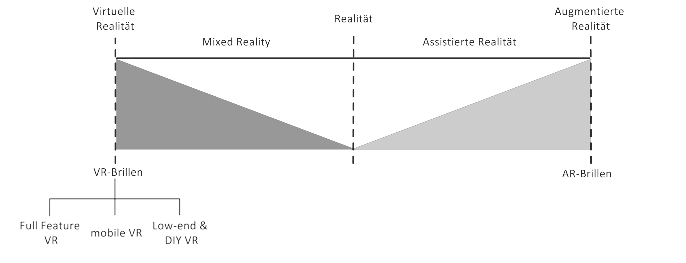
\includegraphics[width=1\textwidth]{data/bilder/VRvsAR.pdf}
    \caption{Einordnung von Smartglasses \cite[S.~28]{ThomasDirkMetzgerHelmutNiegemannHrsg2018}}
    \label{fig:Einordnung_Von_Smartglasses}
\end{figure}


\end{comment}
%
\subsection{Virtual Reality}
%
\emph{Virtual Reality (VR)} ist das völlige Ersetzen der wahrgenommenen Realität durch eine virtuelle Realität. Dabei wird dem Nutzer das Gefühl vermittelt, \enquote{Teil einer virtuellen Realität zu sein} \cite[S.~22]{ThomasDirkMetzgerHelmutNiegemannHrsg2018}. Virtual Reality-Brillen ermöglichen es dem Nutzer im Gegensatz zu Augmented Reality-Brillen komplett in eine virtuelle Realität zu wechseln. Realisiert wird dies durch vollständig geschlossene Gehäuse und Linsen, die vor dem Bildschirm befestigt sind. Mittels der Linsen vor dem Display wird ein scharfes Sehen in einem sehr nahen Bereich ermöglicht. Bei VR-Brillen wird zwischen Full-Feature, Mobile und Low-Budget VR-Brillen unterschieden. Full-Feature Brillen wie die Oculus Rift (Abbildung \ref{fig:OculusRift}) sind mit einer für jedes Auge separaten Full-HD-Auflösung mit hoher Bildwiederholungsrate ausgestattet und bieten dank einer leicht versetzten Anordnung einen dreidimensionalen Effekt. Mobile- und Low-Budget-VR-Brillen wie die Samsung Gear sind Produkte, die mithilfe eines aufgesetzten Smartphones eine Virtuelle Realität erstellen.
%
\begin{figure}[htbp]
    \centering
    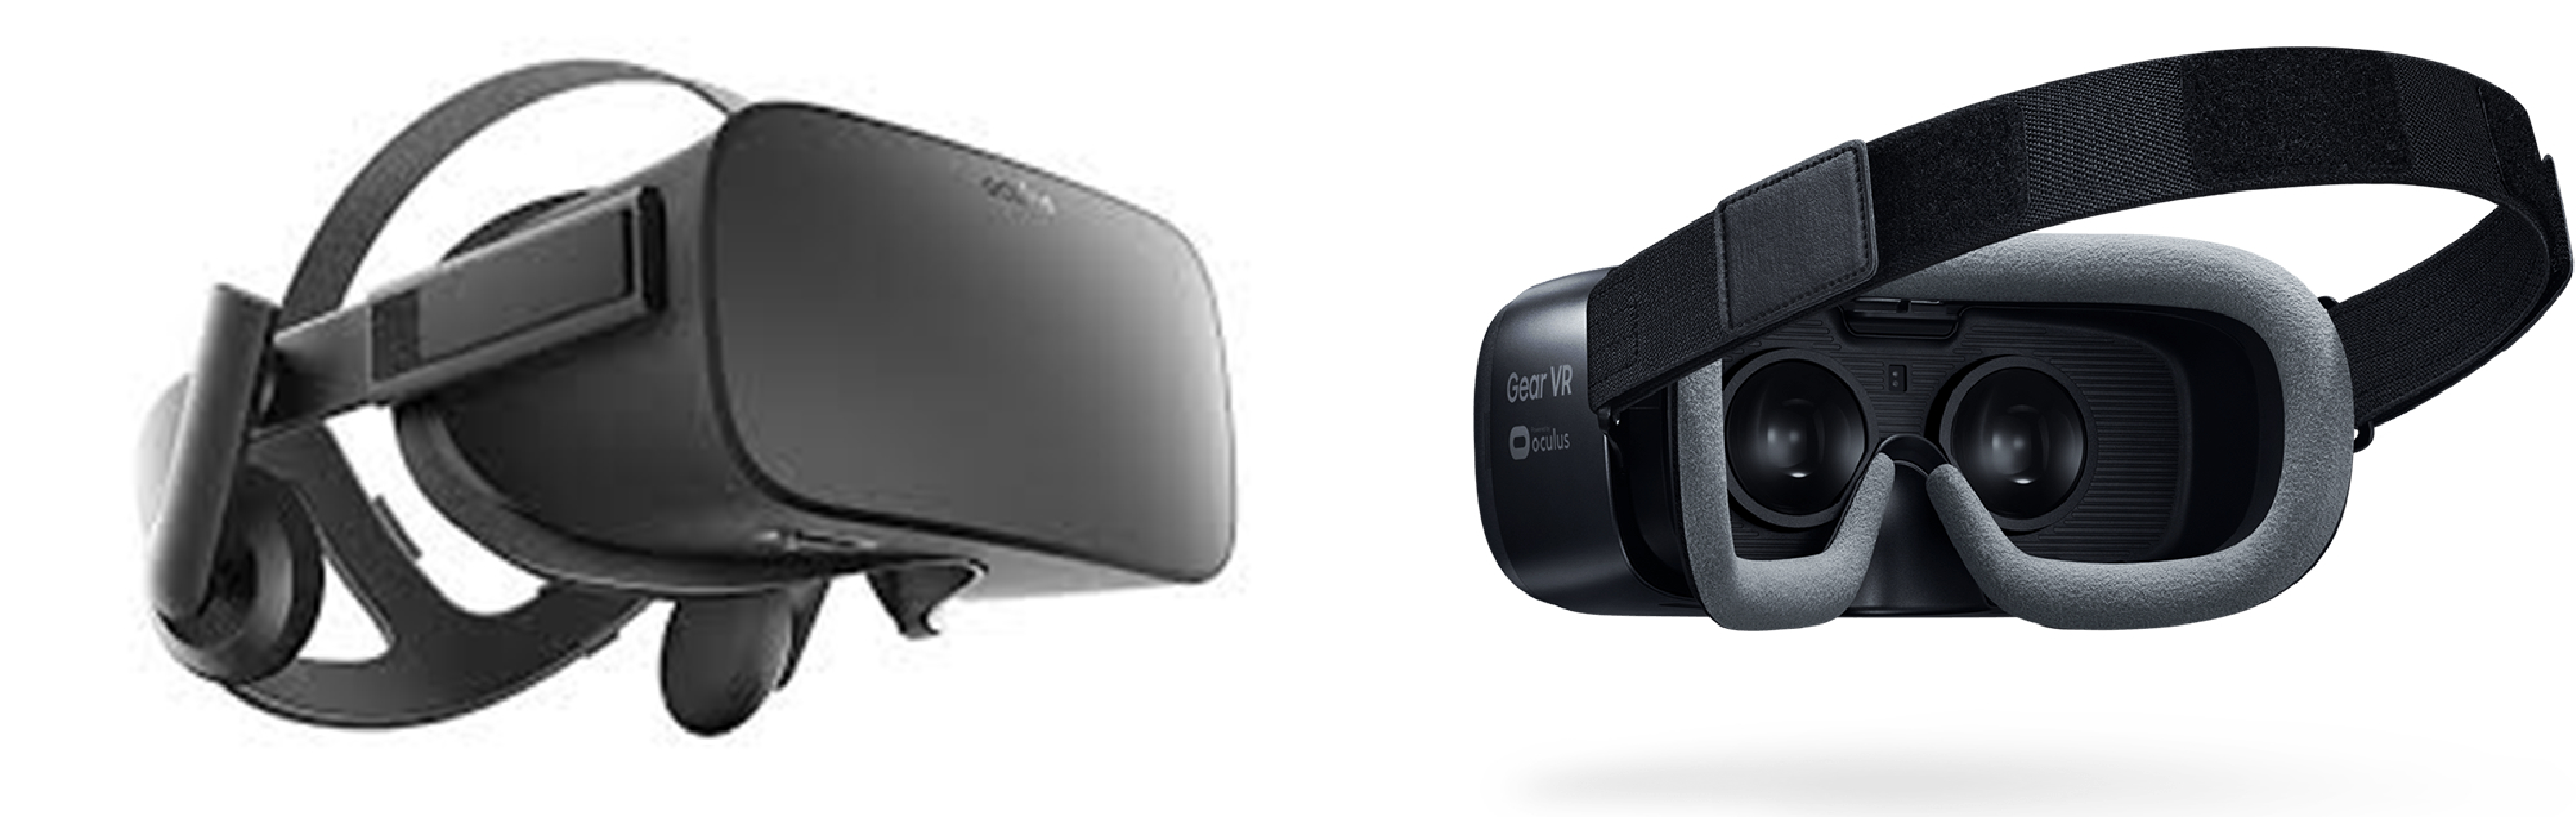
\includegraphics[width=1\textwidth]{data/bilder/Rift_Gear.pdf}
    \caption{Oculus Rift \cite{Oculus2018} (links) und Samsung Gear \cite{Samsung2018} (Rechts)}
    \label{fig:OculusRift}
\end{figure}
%

Der Anwender verliert durch diese Brillen das Gefühl, auf einen Bildschirm zu schauen. Die Außenwelt wird vollkommen ausgeblendet. Bewegungen mit dem Kopf werden automatisch in die virtuelle Welt übernommen. Nutzer bekommen das Gefühl, vollständig Teil der virtuellen Welt zu sein \cite[S.~22ff]{ThomasDirkMetzgerHelmutNiegemannHrsg2018}. 
%
\subsection{Augmented Reality}
%
\emph{Augmented Reality (AR)} ist im Gegensatz zu Virtual Reality das Einblenden von Informationen in das direkte Sichtfeld des Nutzers. Das Blickfeld des Trägers wird also um virtuelle Informationen erweitert \cite[S.~26]{Schwenke2016}. Es wird keine komplett virtuelle Realität erzeugt, sondern die reale Welt um digitale Inhalte ergänzt. Es gibt  unterschiedliche Arten von Brillen, die Augmented Reality-Effekte erzeugen. Differenziert wird zwischen Brillen, die \enquote{echte} Augmented Reality erzeugen und denen, die \emph{unterstützende Realität} erzeugen.

%
\subsubsection{Mixed Reality}
%
Unter \emph{Mixed Reality} wird eine Vermischung von realer Umgebung und virtueller Realität verstanden. Dabei wird eine Umgebung erstellt, in der reale und virtuelle Objekte kombiniert werden können. Objekte oder Personen der realen und virtuellen Welt können miteinander interagieren \cite{Schanze2017}. Diese Form der \enquote{echten} Augmented Reality wird durch Brillen wie die Microsoft Hololens erzeugt. Dabei werden kontextsensitive Informationen direkt im Sichtfeld des Nutzers eingeblendet. Oberflächenerkennung ermöglicht eine Verschmelzung von realer Welt und digitalen Informationen. Die Microsoft Hololens (Abbildung \ref{fig:Microsoft_Hololens}) beispielsweise ist in der Lage, dreidimensionale Hologramme im Sichtfeld des Nutzers anzuzeigen. Dies wird durch zwei transparente Displays ermöglicht. Diese völlige Manipulation der realen Welt wird auch als \emph{Mediated Reality} bezeichnet \cite[S.~46]{Schwenke2016}.
%
\begin{figure}[htbp]
    \centering
    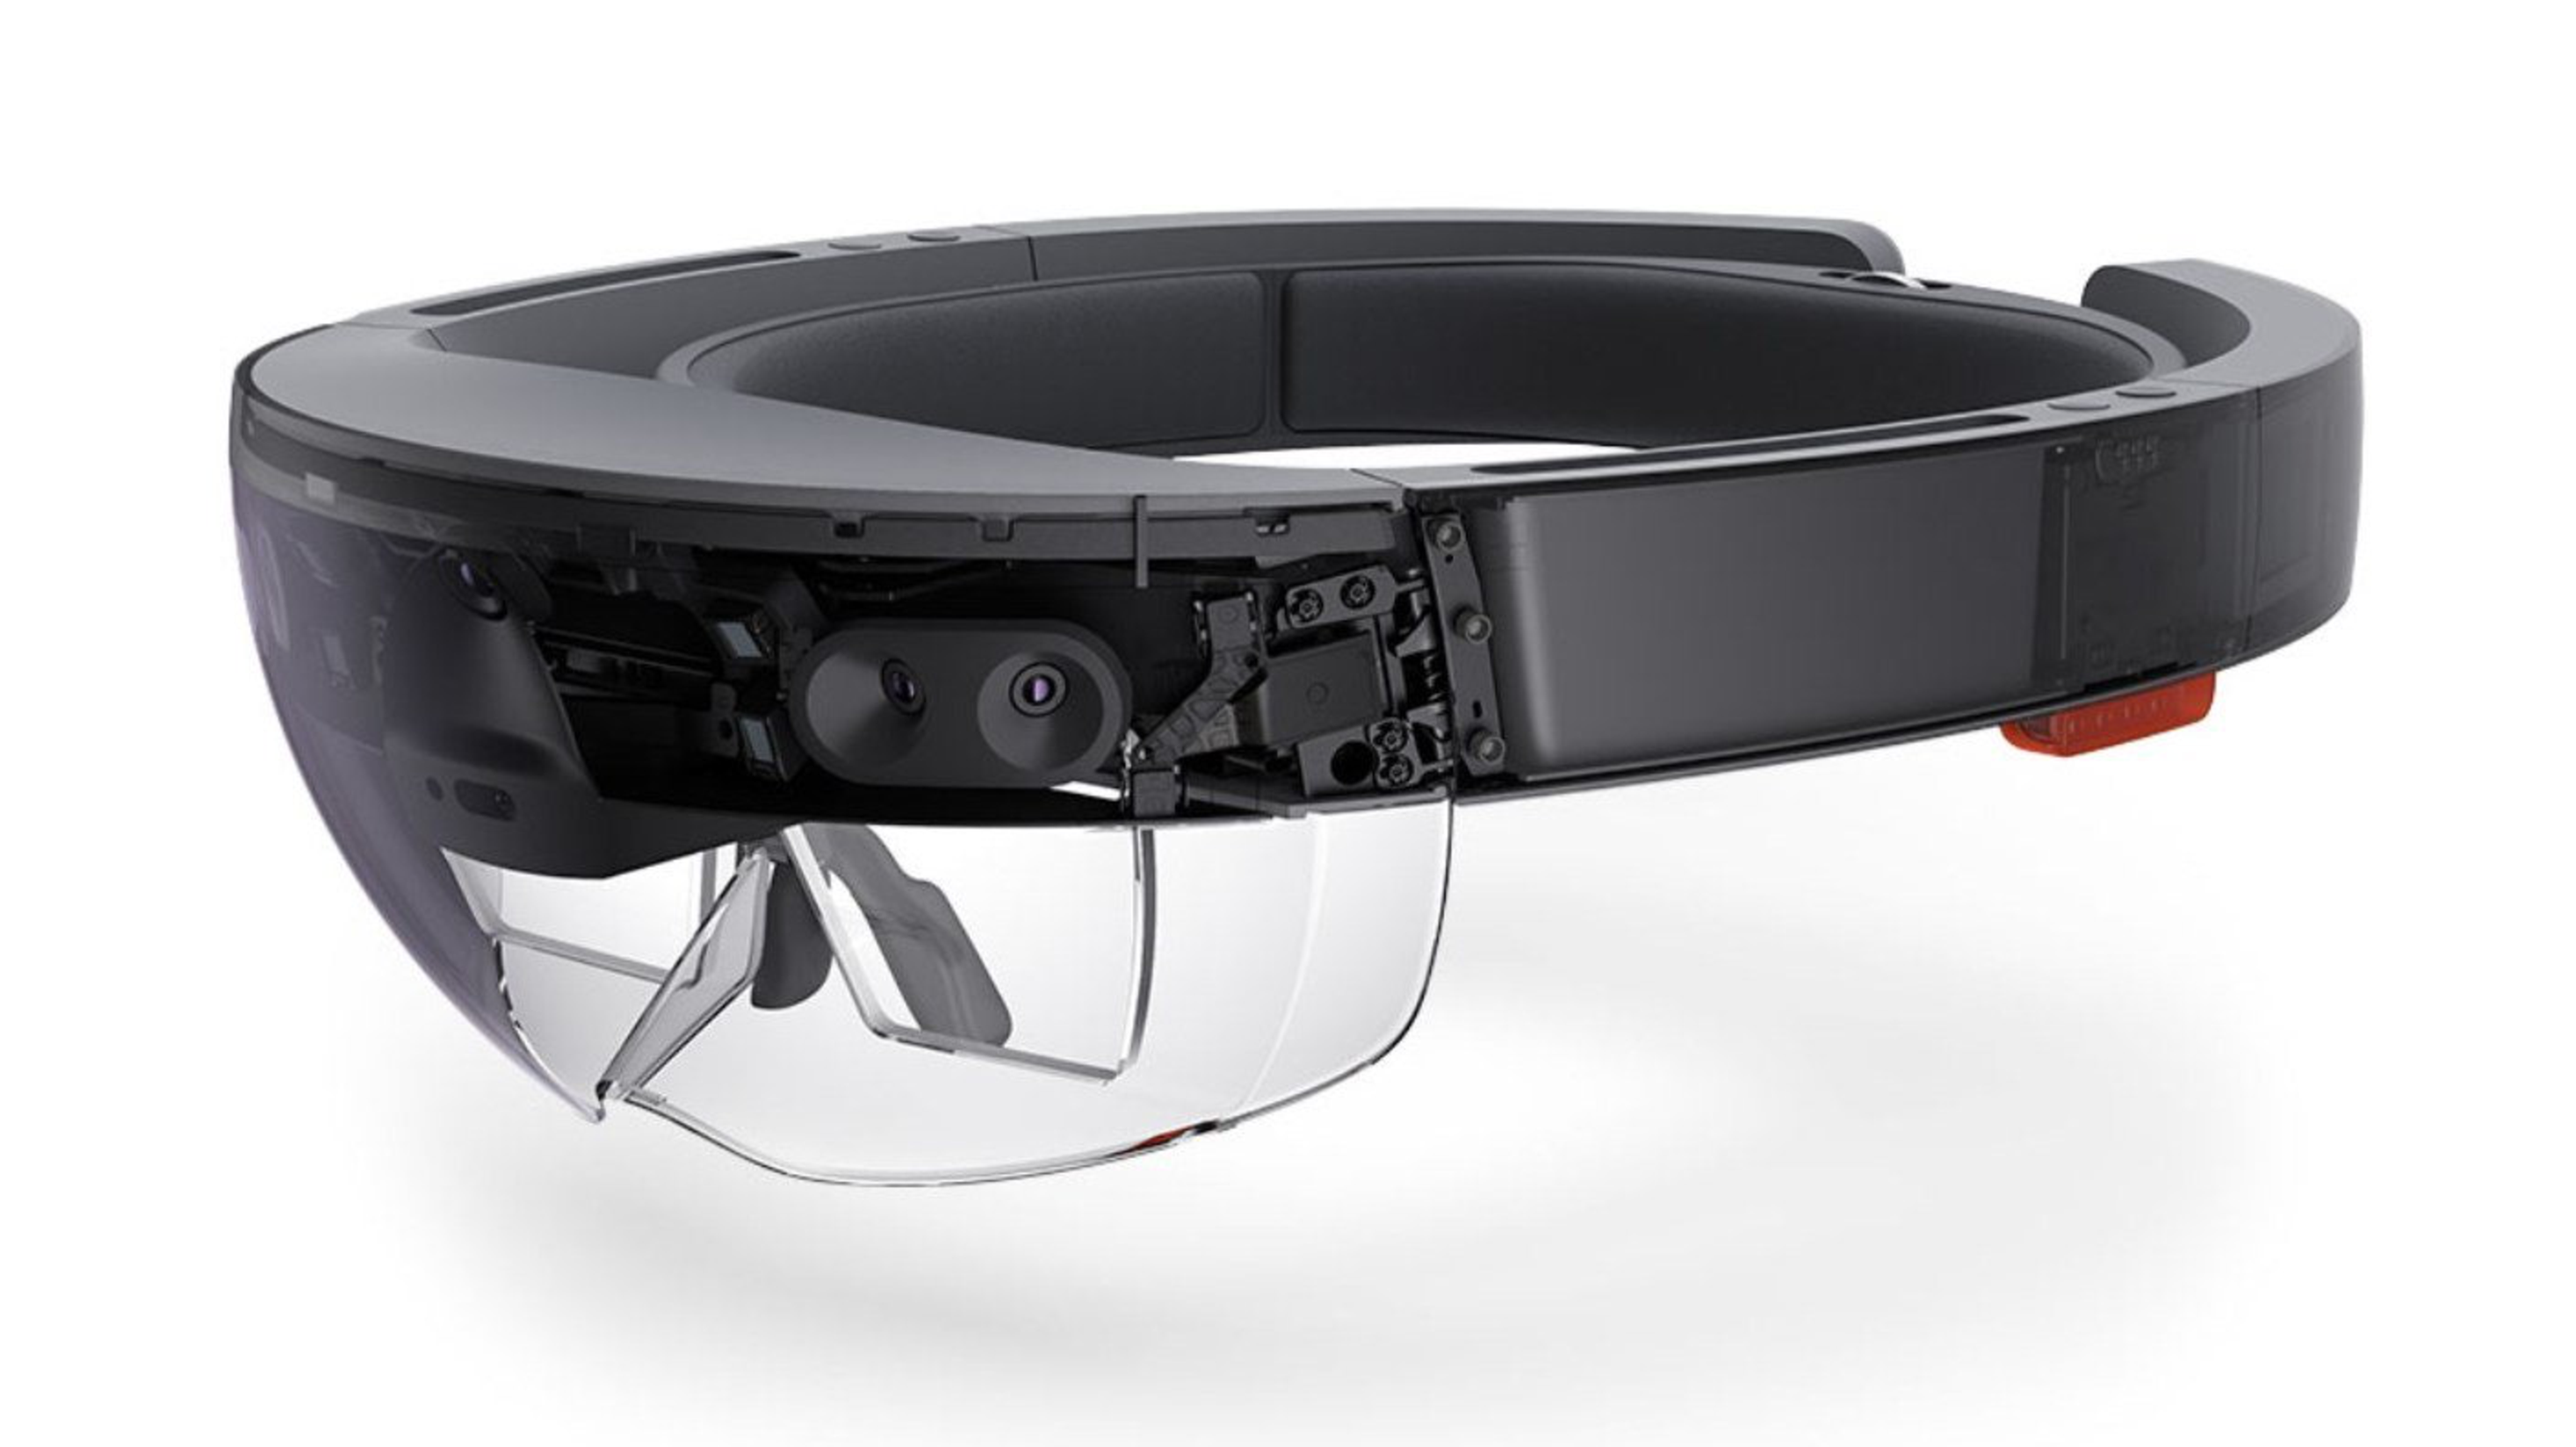
\includegraphics[width=0.5\textwidth]{data/bilder/Microsoft_Hololens.pdf}
    \caption{Microsoft Hololens \cite{O.V.}}
    \label{fig:Microsoft_Hololens}
\end{figure}
%
%

\subsubsection{Assistierte Realität}
\label{sec:AssistierteRealitaet}
%
Von \enquote{echter} AR abzugrenzen ist eine \emph{assistierte Realität}, die beispielsweise durch die \emph{Google Glass}, die \emph{Realwear hmt1} oder die \emph{Epson Moverio BT-200} (vgl. Kapitel \ref{sec:VergleichSmartglasses}) erzeugt wird.

Viele dieser Brillen werden mittels eines sogenannten \emph{Optical Head Mounted See-Through-Displays} \cite[S.~26]{Schwenke2016}, einem Prisma auf einem Auge, virtuelle Inhalte angezeigt, ohne Verlust der Realität mit sich zu ziehen. Bei manchen Assisted Reality-Brillen ist dieses Display jedoch nicht transparent. Es wird lediglich ein kleines Display vor dem Auge angeordnet (vgl. Realwear hmt-1, Kapitel \ref{sec:Realwear_hmt-1}). Im experimentellen Zustand befinden sich Geräte, die Informationen statt auf ein transparentes Display direkt auf die Retina des Auges projizieren \cite[S.~241]{Broll2013}. Ebenfalls zu erwähnen sind am Anfang ihrer Entwicklung befindliche Kontaktlinsen, sogenannte \emph{Smartlenses}, die Informationen mittels LEDs direkt auf die Kontaktlinse bzw. Netzhaut projizieren sollen \cite{Donath2014, Schwan2014}. Im medizinischen Bereich werden bereits heute sub-retinale Implantate getestet, die es ermöglichen, beschädigte Nerven zu ersetzen \cite{Young2013}. Dies ermöglicht ebenfalls die Einblendung von assistierten Realitäten.

Steuern lassen sich AR-Brillen mittels Objekterkennung durch die Kamera (bspw. Gestensteuerung) oder mobiler Hilfsmittel wie Headsets (\emph{Pick-by-Voice}) \cite{INTRALOGISTIK2016}. Es ist also möglich per Gesten- oder Sprachsteuerung zu navigieren. Manche Smartglasses besitzen zudem Touch-Sensoren.

Der Einsatz weiterer Sensoren, wie Trägheitssensoren oder Standortbestimmung sind ebenfalls möglich. Die Kamera einer solchen Smartglass kann zudem über weitere Sensoren, wie Termalsicht, verfügen \cite[S.~27]{Schwenke2016}. Oftmals sind diese Smartglasses mit WLAN, Mobilfunk oder Nahfeldtechnologien mit dem Internet verbunden oder über Schnittstellen mit einem externen Smartphone verknüpft, welches diese Funktionalitäten bereitstellt \cite[S.~28]{Schwenke2016}.

Für Augmented Reality sind Smartglasses zwar nicht zwingend erforderlich, da diese auch mittels bspw. Smartphones erreicht werden kann. So zeigt Apple mit dem AR-Kit \cite{Apple2018} die technischen Möglichkeiten mittels Augmented Reality in Smartphones. Es ist möglich mit dem Ende 2018 in iOS 12 erscheinenden AR-Kit 2 mit mehreren Nutzern in einer virtuellen über den realen Raum gelegten Realität zu interagieren. Smartglasses bieten jedoch viele Vorteile, da diese die Hände frei halten und die erweiterte Realität direkt vor den Augen des Betrachters und nicht in einem in der Hand befindlichen Smartphone dargestellt wird.

Softwaretechnische Beschränkungen der Smartglass sind grundsätzlich die gleichen, die auch für Android-Smartphones gelten. Auf allen gängigen Assisted Reality Smartglasses befindet sich als Betriebssystem Android (vgl. Kapitel \ref{sec:VergleichSmartglasses}). Weitere Beschränkung erfahren Smartglasses lediglich durch die geringe Displaygröße, die eine starke Anpassung einer Anwendung erfordert (siehe Kapitel \ref{sec:Grenzen_des_Einsatzes_von_Smartglasses}).
%
%
%
% - - - - - Vergleich verschiedener Smartglasses - - - - - - - - 
%
%
%
\section{Vergleich verschiedener Smartglasses}
\label{sec:VergleichSmartglasses}
% 2 Seiten
Da in dieser Arbeit Augmented Reality-Brillen und insbesondere Smartglasses mit assistierter Realität (\ref{sec:AssistierteRealitaet}) behandelt werden, werden im Folgenden einige Brillen dieses Bereiches vorgestellt.
%
%
%
% - - - - - - - - Google Glass - - - - - - - - - - - -
%
%
%
\subsection{Google Glass}
\label{sec:Google_Glass}
Der 2012 eingeführte Prototyp einer ersten Version von Google Glass (\enquote{Explorer Edition}) hat ein über dem rechten Auge plaziertes durchsichtiges quaderförmiges Display. Neben dem Display befindet sich eine hochauflösende Kamera sowie ein Mikrofon. Im Bügel der Brille ist die Recheneinheit angeordnet. Die Batterieleistung der Brille betrug beim ersten Prototypen nur wenige Stunden, ist in neueren Versionen jedoch deutlich erhöht worden \cite{Inc.2018}. Die Brille ist mit WLAN ausgestattet und ermöglicht mittels einer Verknüpfung mit einem Smartphone die Verbindung ins Mobilfunknetz sowie die Standortbestimmung mittels GPS.
%
\begin{figure}[htbp]
    \centering
    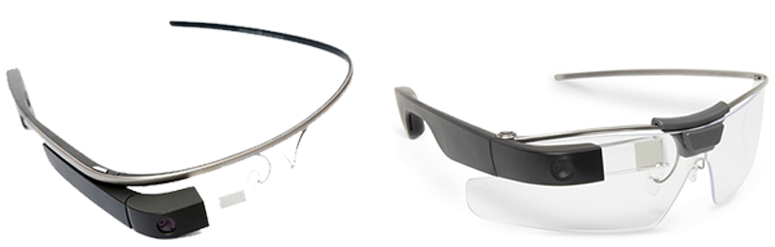
\includegraphics[width=0.8\textwidth]{data/bilder/Glass_1_und_2.png}
    \caption{Google Glass 1 (\enquote{Explorer Edition}) \cite{Reckmann2014a} (links) und Glass Enterprise Edition \cite{Huvelin2017} (rechts)}
    \label{fig:GlassModel}
\end{figure}
%

Die Brille lässt sich über verschiedene Sensoren steuern. So besitzt sie ein Touchpad im Bügel der Brille. Sprachbefehle ermöglichen ebenfalls die Steuerung der Brille. Augenbewegungen des Nutzers werden durch einen Infrarotsensor erfasst, sodass eine Auswahl von Elementen im User-Interface per Augensteuerung möglich ist. Die Kameraaktivität wird nicht angezeigt \cite[S.~30]{Schwenke2016}. Die Glass ist mit einem Android-Betriebssystem ausgestattet. Es gibt eine ausführliche Dokumentation mit speziellen APIs zur Entwicklung spezieller Glass-Anwendungen \cite{Google2018b}.

Mittlerweile hat Google eine speziell für den professionellen Einsatz optimierte Brille veröffentlicht, die \enquote{Glass Enterprise Edition} \cite{Inc.2018}. Diese Brille ist nur für den professionellen Einsatz zugelassen und wird nicht an Privatpersonen verkauft. 
%
%\insertMore{Unterschiede Glass Enterprise-Personal }
%
%
%
% - - - - - Epson Moverio BT-200 - - - - - - - - 
%
%
%
\subsection{Epson Moverio BT-200}
\label{sec:Epson_Moverio_BT-200}
Die Smartglass \emph{Moverio BT-200} von Epson hat im Gegensatz zur Google Glass zwei Bildschirme (je ein Bildschirm vor jedem Auge). 
%
\begin{figure}[htbp]
    \centering
    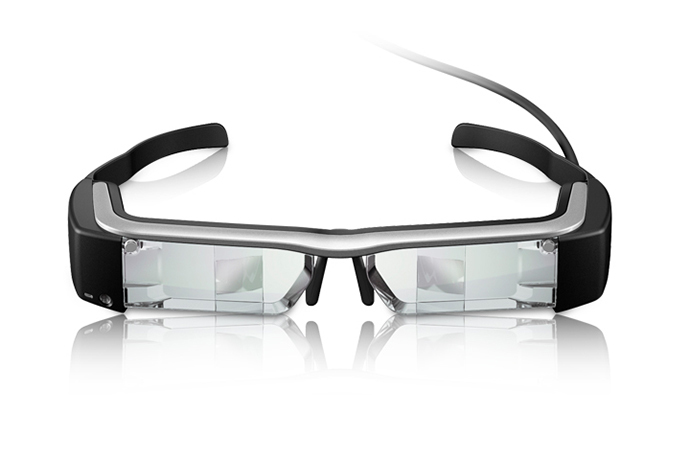
\includegraphics[width=0.4\textwidth]{data/bilder/Moverio_BT-200.png}
    \caption{Epson Moverio BT-200 \cite{Epson}}
    \label{fig:BT-200}
\end{figure}
%
Der Prozessor sowie die Batterie sind extern mittels eines Kabels mit der Brille verbunden. Die Brille verfügt über ein Touchpad, welches ähnlich dem der Google Glass am Bügel der Brille befestigt ist. Die Kamera der Brille ist deutlich geringer aufgelöst (640x480 Pixel), zeigt die Benutzung jedoch im Gegensatz zur Google Glass über eine kleine Leuchtdiode an. Wie auch bei der Google Glass ist das Betriebssystem der Moverio BT-200 Android \cite[S.~32]{Schwenke2016}. Diese Smartglass ist momentan nur in einer Developer-Edition erhältlich \cite{Epson}.
%
%
%
% - - - - - Vuzix M300 - - - - - - - - 
%
%
%
\subsection{Vuzix M300}
\label{sec:Vuzix_M300}
Die \emph{Vuzix M300} ist speziell für den professionellen Einsatz konzipiert. Sie verfügt über ein nicht-transparentes Display am rechten Auge, hat eine HD-Kamera und großen internen Speicher. Sie ist spritzwassergeschützt und nach Herstellerangaben robust gestaltet. Die Brille verfügt über ein Touch Pad sowie zwei Mikrofone zur Sprachsteuerung. 
%
\begin{figure}[htbp]
    \centering
    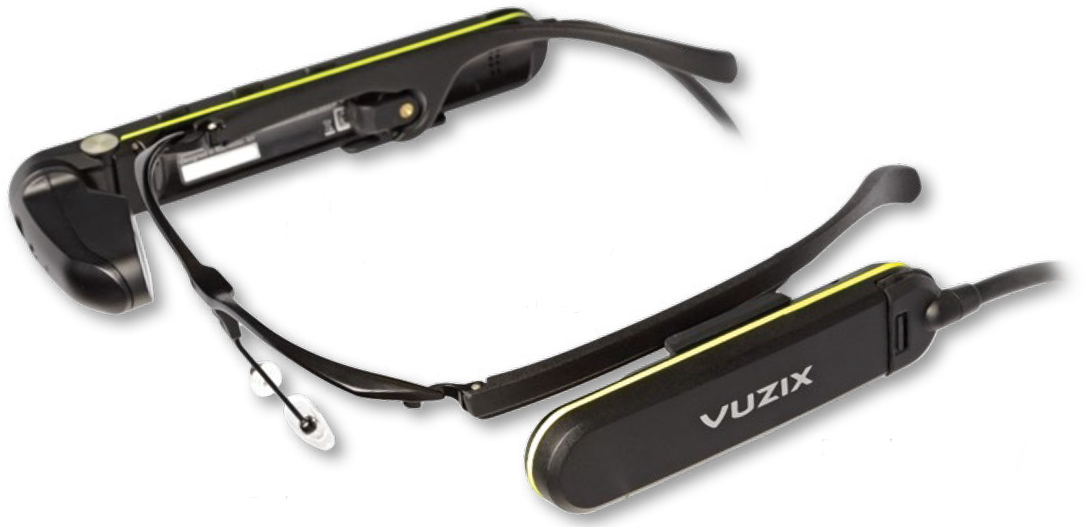
\includegraphics[width=0.4\textwidth]{data/bilder/m300-top.png}
    \caption{Vuzix M300 \cite{Vuzix2018}}
    \label{fig:Vuzix_M300}
\end{figure}
%

Die Vuzix M300 verfügt über schnell austauschbare Akkus, die je nach Anwendungszweck dynamisch angesteckt werden können. So gibt es je nach Anforderung verschieden schwere Akkus. Dies ermöglicht den Einsatz der Brille über einen beliebig langen Zeitraum.

Das Betriebssystem der Brille ist ebenfalls Android. Es lassen sich grundsätzlich alle für Android 6 konzipierten Apps auf der Brille bedienen, jedoch auch speziell für die Brille entwickelte Apps. Die Brille kann mit iOS- und Android-Smartphones gekoppelt werden, um Zugriff auf GPS und Mobilfunk zu erhalten. Zur Entwicklung für die App steht Entwicklern eine weitreichende Dokumentation sowie spezielle APIs zur Verfügung. \cite{Vuzix2018}
%
%
%
% - - - - - Realwear hmt-1 - - - - - - - - 
%
%
%
\subsection{Realwear hmt-1}
\label{sec:Realwear_hmt-1}
%
\begin{figure}[htbp]
    \centering
    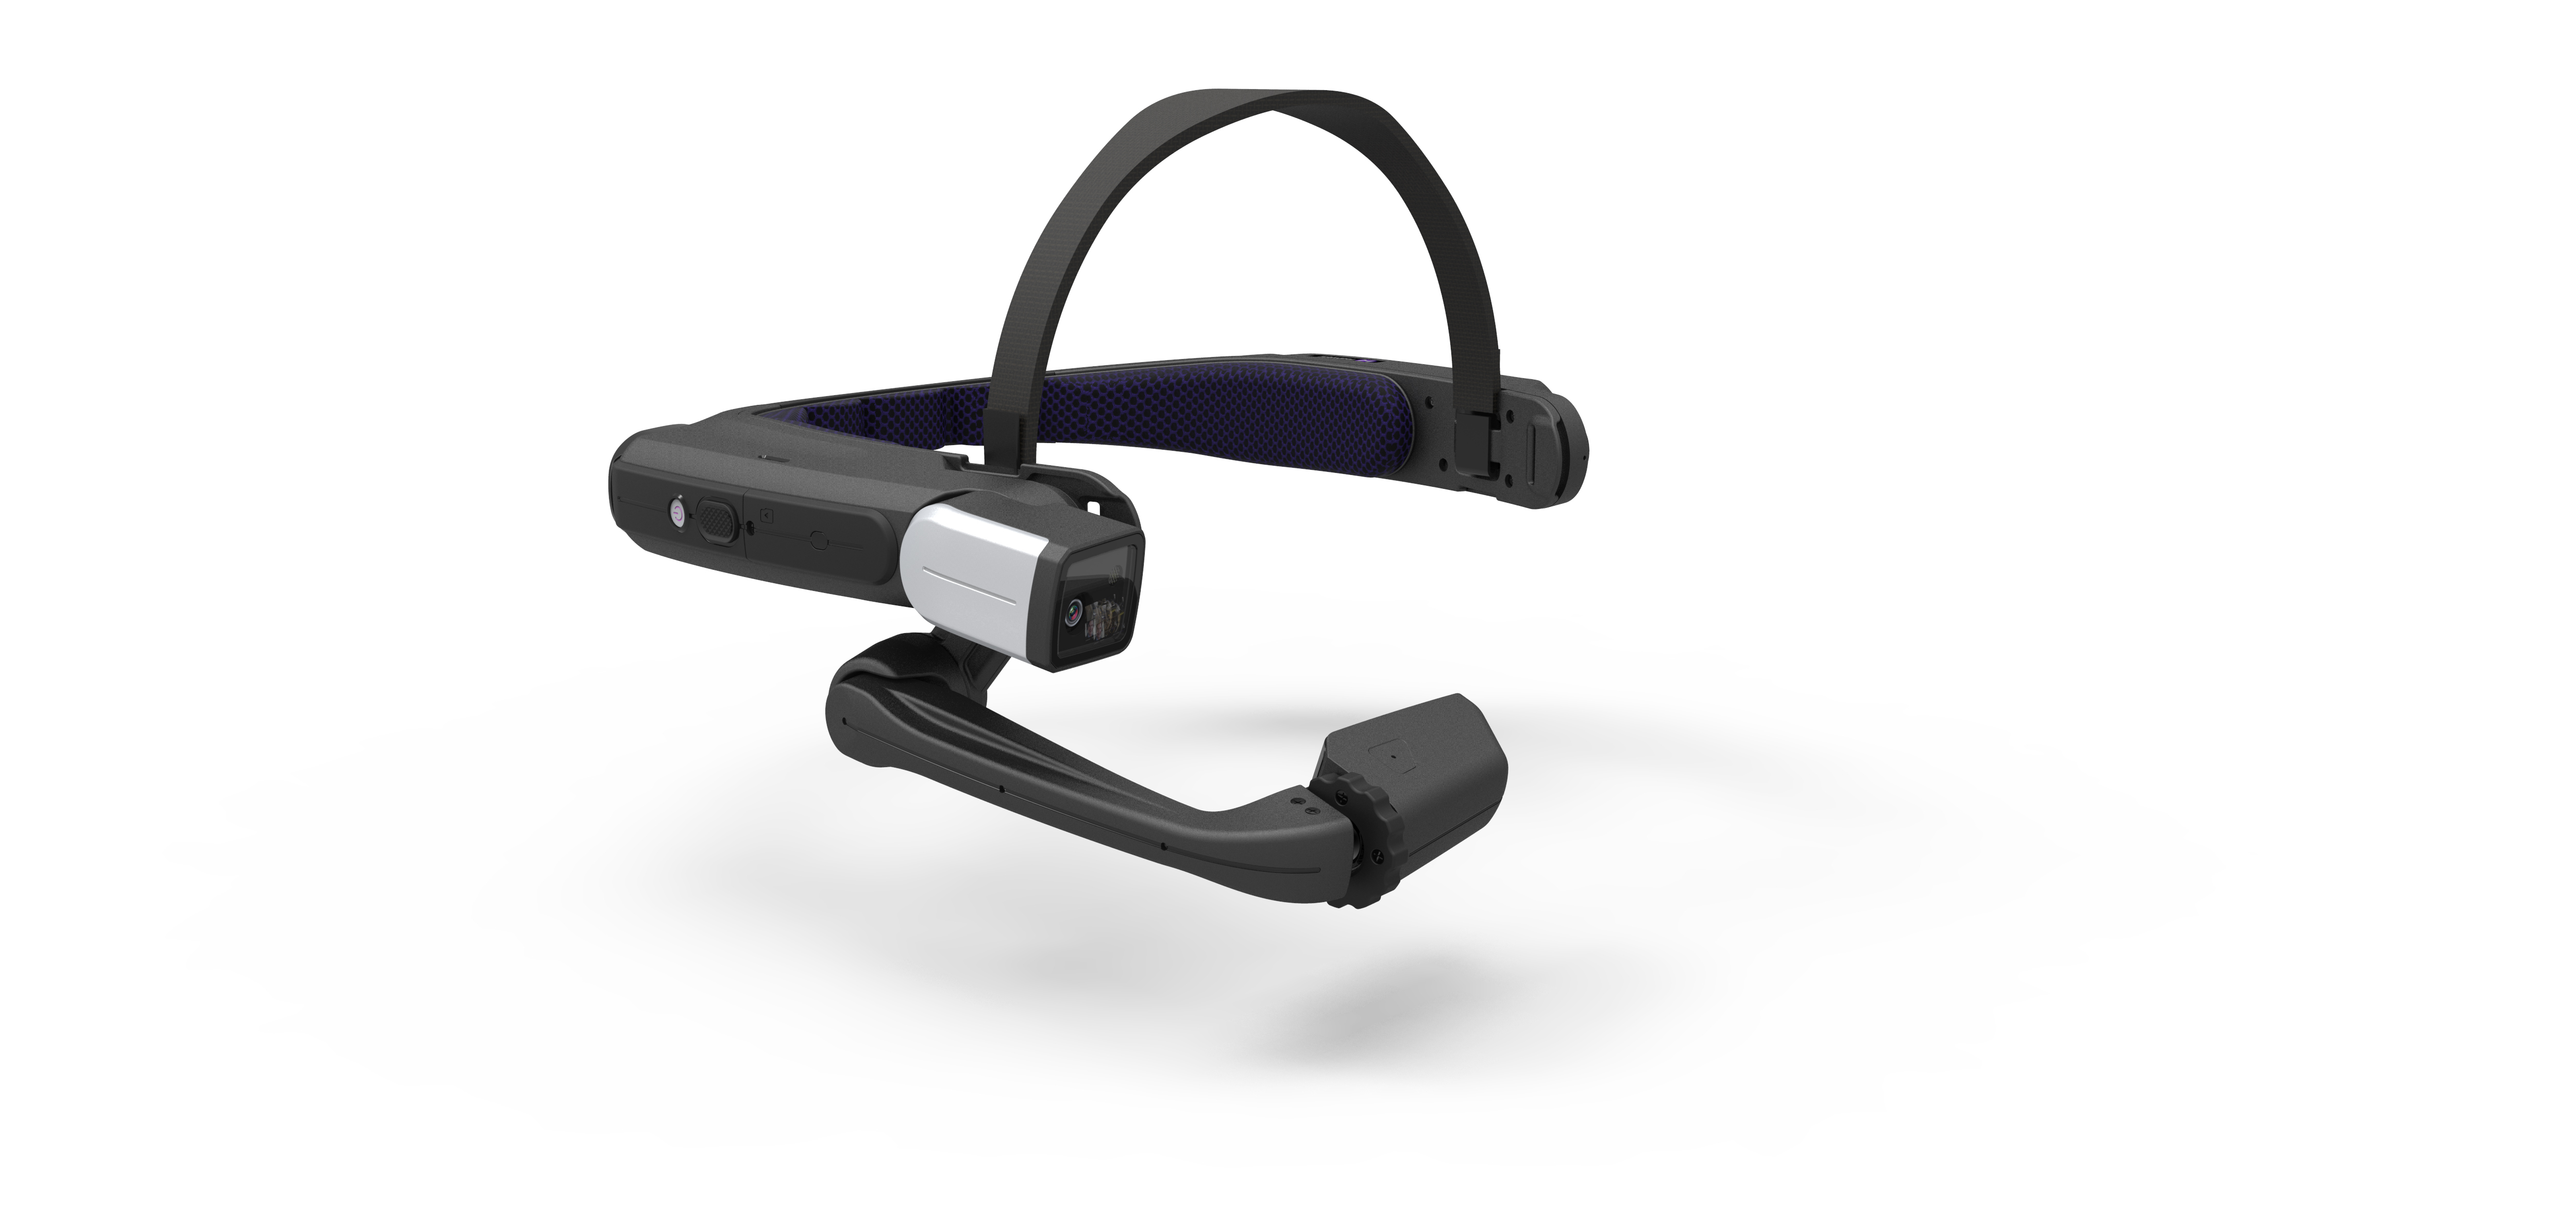
\includegraphics[width=0.9\textwidth]{data/bilder/HMT_1.jpg}
    \caption{Realwear hmt-1 \cite{Wire2017}}
    \label{fig:hmt1}
\end{figure}
%

Die \emph{Realwear hmt-1} ist ebenfalls für den professionellen Einsatz optimiert. Ähnlich der Google Glass ist ein Display über dem rechten Auge befestigt. Dazu kann der Bügel mit dem Display sowohl über dem linken wie auch dem rechten Auge befestigt werden.

Im Gegensatz zur Glass ist dieses Display jedoch nicht transparent, es ist jedoch für den Außeneinsatz konzipiert und ist auch bei starkem Sonnenlicht nutzbar. Die Brille ist vollständig abwischbar. Sie erfüllt dazu den IP66-Standard \cite{Realwear2018}.

Prozessor und Batterie sind im Bügel der Brille befestigt. Die Brille  besitzt eine Sprachsteuerung mit integrierter Noice-Cancellation mittels vier eingebauter Mikrofone. Die Batterie der Brille hält einen gesamten Arbeitstag. Im Gegensatz zur Glass und BT-200 ist die hmt-1 so ausgelegt, dass sie Stürze aus 2~m Höhe auf Betonboden übersteht. Wie auch Glass und BT-200 ist das Betriebssystem der hmt-1 Android. Es gibt eine gut dokumentierte Entwicklerdokumentation und APIs zur Entwicklung von speziell für die Brille konzipierten Android-Anwendungen \cite{Realwear2018}.
%
%
%
% - - - - - Smartglasses im beruflichen Umfeld - - - - - - - - 
%
%
%
\section{Smartglasses im beruflichen Umfeld}
\label{sec:Smartglasses_im beruflichen_Umfeld}
% 3 Seiten
Die Logistikbranche ist Deutschlands drittgrößte Branche \cite{Zobel2016}. In der Logistikbranche werden Datenbrillen in Form von Assistierten AR-Brillen eingesetzt \cite{Niemoller2017}.
\\
Smartglasses ermöglichen die Digtialisierung von Arbeitsprozessen und machen es möglich, die Integration von Mitarbeitern in Unternehmensprozesse zu verbessern \cite{Zobel2016}. Sie liefern kontextabhängige Informationen, beispielsweise durch das Einlesen von Barcodes bzw. QR-Codes. Angestellte der Logistikbranche der Transportlogistik werden so in Echtzeit mit Informationen, wie beispielsweise Lieferaufträgen versorgt. In einer Use-Case-Studie von Niemöller \cite{Niemoller2017} wurden insgesamt 36 Einsatzmöglichkeiten für Smartglasses im Logistikdienstleistungssektor ermittelt. Die relevantesten Use-Cases werden im Folgenden dargestellt:
\\
Zum einen wurde das Themenfeld Kommunikation herausgearbeitet. Mittels Smartglasses ist das Anzeigen von Handlungsanweisungen sowie die Darstellung von Videoinformationen mittels Streaming oder Offlinevideos möglich. Eine vereinfachte Kommunikation durch die Übersetzung von Texten ist ebenso möglich. Im Themenfeld Qualitätssicherung ist eine automatisierte Kontrolle mittels einer kamerabasierter Fehlererkennung sowie entsprechender Rückmeldung an den Nutzer möglich. Das Haupteinsatzfeld ist jedoch die Identifizierung anhand gespeicherter Merkmale wie Farbe, Größe und Geometrie oder auch durch die Identifizierung mittels Bar- und QR-Codes \cite{Niemoller2017}. Identifizierung von Objekten ermöglicht die Anzeige von Zusatzinformationen. Im Themenfeld Sicherheit ist die kontextabhängige Darstellung von Sicherheits- und Warnhinweisen möglich. 

Auf dem Fachkongress \emph{Smart Glasses Experience Days} \cite{Manokaran-Pathamathan2017} wurden weitere Einsatzfelder aufgezeigt. So können über die Datenbrille Montage- oder Reparaturanleitungen angezeigt werden. Zwecks Dokumentation werden Arbeitsschritte und Informationen des vorhergehenden Angestellten angezeigt. Per Remoteunterstützung können Angestellte Hilfe bei komplizierten Arbeitsschritten erhalten. Für Lagermitarbeiter können Anweisungen angezeigt werden, wie und in welcher Reihenfolge Anweisungen befolgt werden sollen.

Neben der Logistikbranche werden Smartglasses auch in anderen Branchen eingesetzt. In dem Studienbericht \emph{Smart Glasses in der Produktion} des Fraunhofer-Instituts für Produktionstechnologie IPT von 2016 \cite{Plutz} wurde der Einsatz von Smartglasses im beruflichen Umfeld der industriellen Produktion analysiert. So setzen 3,4\% der 237 befragten Unternehmen  Smartglasses bereits ein. 15,1\% wollen diese in nächster Zeit einsetzen. Die häufigsten Anwendungsgebiete waren Mitarbeiterschulungen (27,3\%), Fernwartung/Videotelefonie (27,1\%), Echtzeitanzeige von Informationen (22,8\%) und industrielle Bildverarbeitung (17,5\%). Laut dem Bericht ist es möglich, nicht nur prozessrelevante Informationen zur Verfügung zu stellen, sondern Angestellte auch dazu zu befähigen, Informationen prozessintegriert zu erzeugen. Zudem sei es möglich, hoch aufgelöste Zeiterfassung manueller Tätigkeiten zu realisieren und Prüfdaten nicht wie bislang handschriftlich zu erfassen, sondern dabei die Hände frei zu haben.

Laut einer Pressemitteilung des Logistikunternehmens DHL vom 2. August 2017 führt der Einsatz von Smartglasses zu einer 15-prozentigen Produktivitätssteigerung bei geringerer Fehlerquote \cite{DeutschePostDHLGroup2017}. Mittels Sprachsteuerung lassen sich einzelne Kommissionieraufträge aufrufen und die nötigen Informationen auf dem Display anzeigen. So ist es möglich, Lagerort, Lagerplatz und die zu packende Anzahl der Ware anzuzeigen statt wie bisher auf papierbasierte Auftragsanweisungen zurückzugreifen. 

Das Unternehmen Bosch setzt in ihrer Logistiksparte ebenfalls Smartglasses ein. Für Bosch ist vor allem die Tatsache von Vorteil, dass die Angestellten beim Scannen von Barcodes und QR-Codes freihändig agieren können \cite{Spinger2014}. 
%
\chapter{Anforderungsanalyse}
\section{Ablauf der Medizinprodukteaufbereitung}
\section{Anforderungen bei der Medizinprodukteaufbereitung}
\section{Smartglasses im Bereich der Medizinprodukteaufbereitung}
\subsection{Einsatzmöglichkeiten}
\subsection{Spezifische Anforderungen an Smartglasses im Bereich der Medizinprodukteaufbereitung}
\subsection{Datenschutz}
\subsection{Arbeitssicherheit}
\subsection{Grenzen des Einsatzes von Smartglasses}

%
\chapter{Konzept}
% 0,5 Seiten
%
% - - - - - - - - - - - - - - - - - - - - - - - - 
%
\section{Interaktionsmöglichkeiten}
% 2 Seiten
%
% - - - - - - - - - - - - - - - - - - - - - - - - 
%
\section{Objekterkennung}
% 2 Seiten 
%
% - - - - - - - - - - - - - - - - - - - - - - - - 
%
\subsection{Externe Peripherie}
% 1 Seite 
%
% - - - - - - - - - - - - - - - - - - - - - - - - 
%
\subsection{Medienverwaltung}
% 2 Seiten 
%
% - - - - - - - - - - - - - - - - - - - - - - - - 
%
\section{Medienpräsentation}
% 2 Seiten
%
% - - - - - - - - - - - - - - - - - - - - - - - - 
%
\section{Medienerfassung/-erstellung}
% 2 Seiten
%
%
%
%
% - - - - - Prototyp - - - - - - - - 
%
%
%
\chapter{Prototyp zur Unterstützung in der Sterilgutversorgung}
\label{ch:Prototyp}
In dieser Arbeit wurde ein Prototyp für die \emph{Realwear hmt-1} implementiert. Die Funktionalität, verwendete Technologien sowie die Implementation werden im Folgenden vorgestellt.
%
%
%
% - - - - - Funktionalität des Prototypen - - - - - - - -
%
%
%
\section{Funktionalität des Prototypen}
Mithilfe des Prototypen sind zwei grundsätzliche Funktionalitäten möglich. Es ist einerseits möglich, aus einer bestehenden Liste von Bildergalerien eine Galerie auszuwählen und anzuzeigen. Andererseits kann eine Slideshow in Form einer JSON-Datei per QR-Code von einem Server geladen werden. Innerhalb der Bildergalerie ist es dann möglich, vor und zurück zu navigieren. 
Slideshowauswahl und Slides sind in einer Listenansicht dargestellt, die es ermöglicht, stets 4-5 Elemente auf einmal anzuzeigen und bei Bedarf weitere Elemente nachzuladen. Dies wird mit einem Vor- und einem Zurückbutton realisiert.

Die andere Hauptfunktionalität betrifft Videos. Es ist möglich,  Videos aufzuzeichnen und dieses abzuspielen. Es ist ebenso möglich, einen QR-Code mit einer Adresse auf ein MP4-Video aufzurufen und dieses Video zu streamen. Innerhalb eines abgespielten Videos ist es möglich, 10 Sekunden vor oder zurück zu spulen und zu pausieren. Zudem ist es möglich, Kapitelmarken zu setzen und in einer eigenen Ansicht zu bearbeiten.

All diese Funktionalitäten können via Sprachsteuerung ausgewählt werden. Dazu müssen die Beschriftungen der Buttons laut vorgelesen werden. Die Brille interpretiert dann diese Eingaben als \emph{Click}-Events und ruft entsprechende Funktionen auf.

In der Praxis können Bilder-Slideshow und Videos eingesetzt werden, um Angestellten der AEMP wichtige Informationen zu medizinischen Instrumenten zu geben. So können Hyperlinks zu Anleitungen per QR-Code oder Barcode auf die Smartglass geladen werden und von einem externen Server gestreamt werden.

Um auch ohne Internetverbindung arbeiten zu können, ist es zu Beginn des Appstarts möglich, eine lokale Server-URL per QR-Code einzulesen. Diese wird anschließend vor alle per QR-Code eingelesenen URLs gesetzt, sodass es möglich ist auch in einer Umgebung wie der AEMP, in der keine Internetverbindung zur Verfügung steht, auf Videos und Bilder eines lokalen Servers zuzugreifen. 

Zum Testen wurde ein lokaler NodeJS-Server aufgesetzt, welcher Mediendaten ausliefert.
%
%
%
% - - - - - Verwendete Technologien - - - - - - - - 
%
%
%
\section{Verwendete Technologien}
\label{sec:Verwendete_Technologien}
% 3 Seiten
Für die Implementierung des Prototypen wurde \emph{Android Studio} mit Android in Version 23 verwendet, da dies die neueste Version ist, die von der \emph{hmt-1} unterstützt wird. Die API der \emph{hmt-1} ermöglicht den Zugriff auf die Hardwarefunktionalitäten sowie auf die Sprachsteuerung der Smartglass. Mittels eines Eintrags \emph{\enquote{android:contentDescription}} können Sprachbefehle zu beliebigen Elementen hinzugefügt werden. Die Elemente reagieren dann auf den im Eintrag angegebenen Sprachbefehl und lösen ein \emph{Click}-Ereignis aus.

Die API der Smartglass hat zudem eine Funktionalität, um Barcodes und QR-Codes auszulesen und den Inhalt zurückzugeben und eine API, um Videos in hoher Auflösung aufzuzeichnen. 

Der Prototyp speichert aufgezeichnete Videos auf dem Gerät und serialisiert das dazugehörige Datenobjekt (vgl. Kapitel \ref{sec:Datenmodell}) auf dem Gerätespeicher. Externe Videos und Bilder werden per JSON-Objekt, welches über einen Link von einem Server geladen wird, geladen. Diese JSON-Objekte enthalten alle notwendigen Informationen. So enthält das JSON-Objekt der Slideshow ein Array aus Objekten mit Namen und URL. Beim Video wird der Name, die URL und die Kapitel mit Namen und Position in Millisekunden gespeichert (vgl. Listing \ref{lst:json_video} und \ref{lst:json_slides}).

Der verwendete lokale Server ist ein NodeJs-Server, welcher über die IP-Adresse und den verwendeten Port einen Ordner auf dem Dateisystem freigibt.
%
%
%
% - - - - - Implementation - - - - - - - - 
%
%
%
\section{Implementierung}
\label{sec:Implementation}
Im Folgenden wird die Implementierung des Prototypen beschrieben. 

Das Programm folgt bei der Videofunktionalität dem Model-View-Controller (\emph{MVC})- Pattern, bei dem eine Trennung von Programmlogik, Model und View eingehalten wird.
%
%
%
% - - - - - User-Interface - - - - - - - - 
%
%
%
\subsection{User-Interface (View)}
Die Android-Anwendung wurde nach dem in Abbildung \ref{fig:Storyboard_des_Prototypen} gezeigten Storyboard erstellt. Die Anwendung beginnt in einem Hauptmenü, welches ermöglicht, per Sprachbefehl einen von zwei Buttons auszuwählen. Mit dem ersten Button wird der Nutzer zur Slideshow-Seite weitergeleitet. Beim zweiten Button wird auf die Videoanzeige und beim dritten Button auf die Video-Aufzeichnen Funktion weitergeleitet. Mittels eines \enquote{Schritt-Zurück-Befehls} der Smartglass wird der androidtypische \enquote{Zurückbefehl} betätigt.

\begin{figure}[htbp]
    \centering
    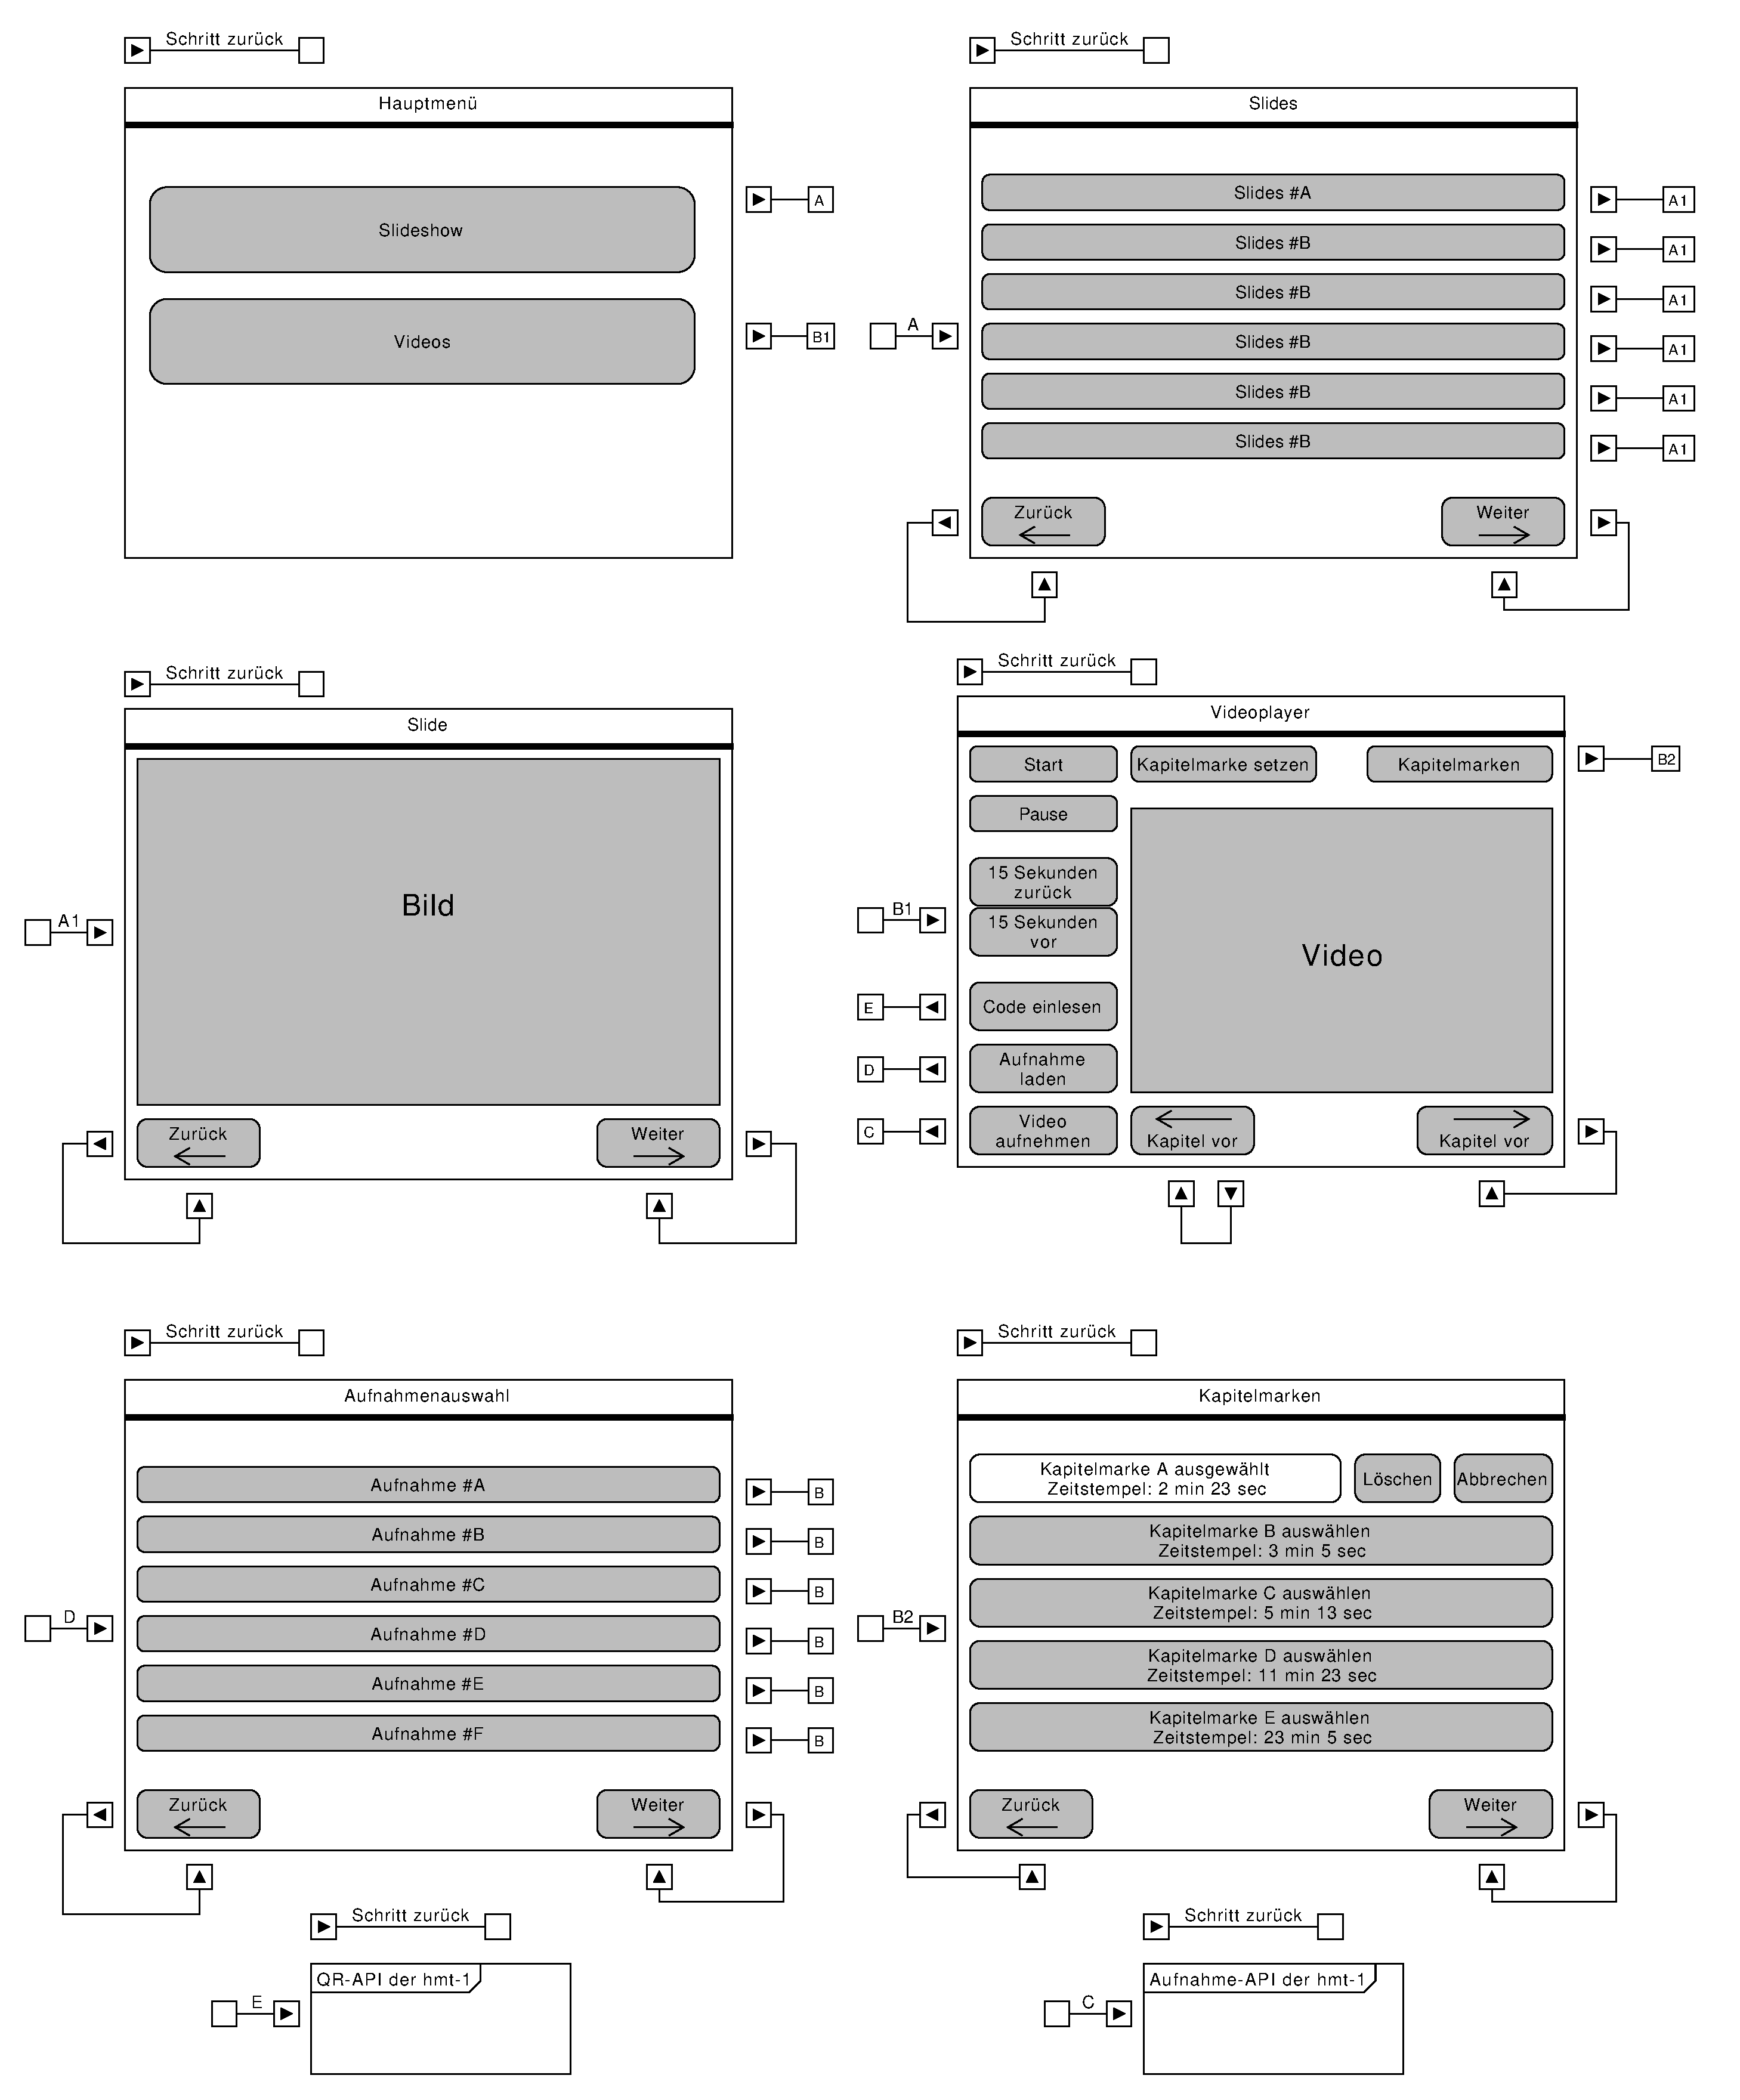
\includegraphics[width=1\textwidth]{data/bilder/UI-Storyboard.pdf}
    \caption{Storyboard des Prototypen}
    \label{fig:Storyboard_des_Prototypen}
\end{figure}

Die Slideshow besteht aus zwei Ansichtstypen. In der ersten Ansicht, welche über das Hauptmenü erreichbar ist, wird eine Liste von Buttons angezeigt, über die einzelne Slides ausgewählt werden können. Am unteren Rand des Fensters ist ein \enquote{Weiterbutton}, welcher die Liste der Buttons aktualisiert, um weitere Slides zur Auswahl zu stellen. Dies ist notwendig, da bei der \emph{hmt-1} klassisches scrollen durch eine Liste nicht möglich ist. Es ist lediglich das Scrollen durch eine kurze Liste per Kopfgesten möglich.

Über einen Button \enquote{Code einlesen} ist es möglich, einen QR-Code zu lesen, der einen Link zu einer JSON-codierten Slideliste kapselt und es so ermöglicht, die Slides dynamisch nachzuladen.

Wird eine Bilderliste ausgewählt, so wird auf eine Unterview verlinkt. Diese besteht aus einer \emph{Image-View} sowie zwei Buttons: \enquote{vorwärts} und \enquote{zurück}. Im Bild wird das aktuelle Bild der Bilderliste angezeigt. Mit \enquote{weiter} wird das nächste, mit \enquote{zurück} das vorherige Bild angezeigt.

Aus der Haupt-Einstiegsview kann zudem die \emph{Videoplayer}-View geöffnet werden. Diese Ansicht besteht aus zwei Bereichen. Links ist eine Sammlung von insgesamt 7 Buttons zum starten und stoppen, vor- bzw. zurückspulen des Videos um 10 Sekunden, Einlesen eines QR-Codes und Einlesen des Videolinks in den Videoplayer. Diese Buttons werden dynamisch ein- bzw ausgeblendet, je nach Stadium, in dem die App sich befindet. So werden immer nur die Buttons angezeigt, die wirklich verwendet werden können. Zusätzlich sind noch zwei Buttons zum Aufnehmen eines Videos und zum Laden einer Aufnahme in den Player. Rechts ist ein Videofenster angebracht, in dem die Videos angezeigt werden.

Einlesen des QR-Codes sowie die Aufnahme des Videos werden mithilfe der API der \emph{hmt-1} realisiert. Der eingelesene Link enthält ein JSON-Objekt, welches den Link sowie die Kapitel enthält. Das Ergebnis wird in der View angezeigt.

Ist ein Video geladen, so werden die Buttons zur Bearbeitung und Verwendung der Kapitelmarken sichtbar. Mittels zweier Buttons an der unteren Bildschirmseite ist es möglich, die jeweils nächsten und vorherigen Kapitelmarken anzusteuern. Mit einem Button an der oberen Bildschirmhälfte ist es möglich, eigene Kapitelmarken an der aktuellen Position des Videos zu setzen. Diese können mittels Spracheingabe benannt werden.

Wird ein Button \enquote{Kapitel} aufgerufen, so wird eine eigene View zur Verwaltung von Kapitelmarken angezeigt, die ähnlich der Slideshowauswahl funktoniert. Hier wird eine Liste angezeigt, in der alle Kapitel aufgelistet werden. Wählt der Nutzer ein Kapitel aus, so erscheinen \enquote{Löschen}- und \enquote{Abbrechen}-Buttons. Mittels \enquote{Löschen} kann das ausgewählte Kapitel gelöscht werden. 
%
%
%
% - - - - - Datenmodell - - - - - - - - 
%
%
%
\subsection{Datenmodell (Model)}
\label{sec:Datenmodell}
In Abbildung \ref{fig:Klassendiagramm} ist neben der Klassenstruktur des Controllers das Klassendiagramm des Models gezeigt. Dieses besteht aus insgesamt vier Klassen: den Basisdatentypen \enquote{Slide}, \enquote{Video} sowie \enquote{VideoChapter} und der Liste von Slides \enquote{SlideList}. 

Die Klasse \enquote{Slide} kapselt einen String \enquote{fileURL} und den Titel \enquote{title}. 
Die Klasse \enquote{VideoChapter} dient zur Speicherung eines Kapitels eines Videos und wird von der Klasse Video verwendet. Ein VideoChapter besteht aus einer Ganzzahl \enquote{position} und dem Namen des Kapitels als String. Die Klasse \enquote{SlideList} kapselt eine \emph{ArrayList} von Slides sowie den Namen der SlideList.
Die Klasse \enquote{Video} besteht aus dem Namen der Datei, in welcher das Video im Dateisystem gespeichert wird, der URL des Videos, dem Titel, sowie aus einer ArrayList von VideoChapter. Video besitzt zudem öffentliche Methoden zum Hinzufügen und Entfernen von Kapiteln sowie zum Persistieren und laden des Video-Models im Dateisystem.
\begin{figure}[htbp]
    \centering
    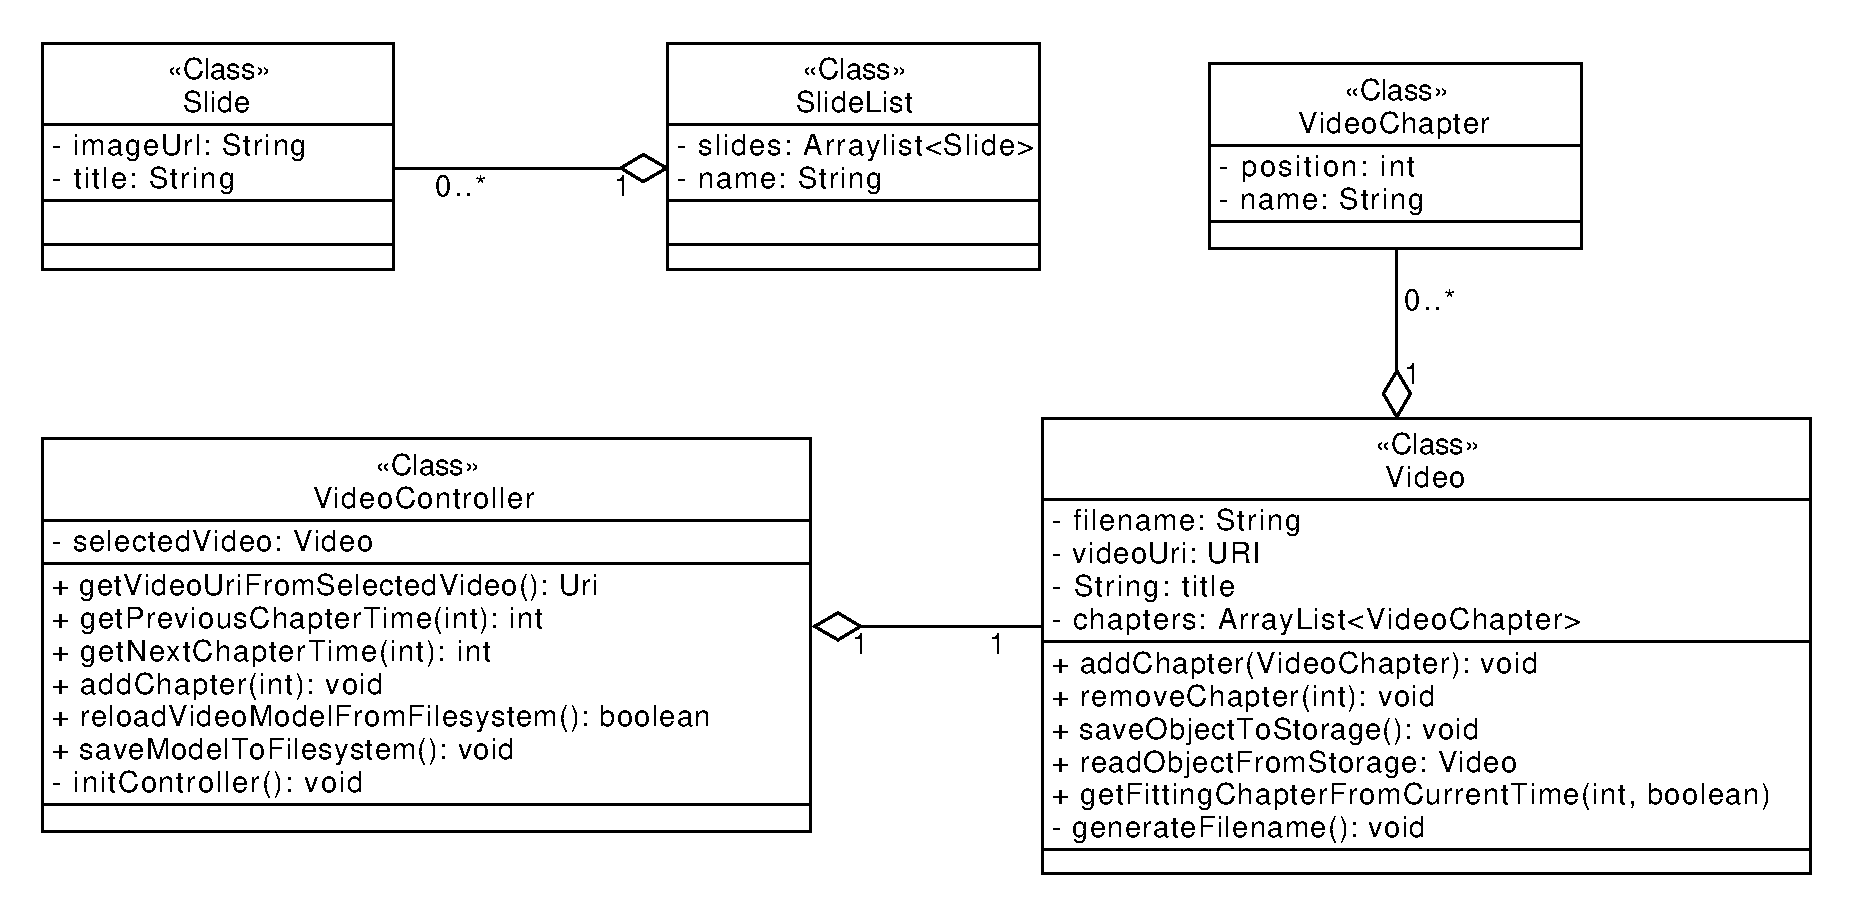
\includegraphics[width=1\textwidth]{data/bilder/Klassendiagramm.pdf}
    \caption{Klassendiagramm der Modelklassen sowie der Controllerklasse}
    \label{fig:Klassendiagramm}
\end{figure}

Die Slides sowie das Video können per Link auf ein JSON-Codiertes Model eingelesen werden. Die Struktur der JSON-Objekte ist in Listing \ref{lst:json_video} und \ref{lst:json_slides} dargestellt.
%
%
%
% - - - - - Programmlogik - - - - - - - - 
%
%
%
\subsection{Programmlogik (Controller)}
Die Programmlogik der Videofunktionalität wird durch einen Controller (vgl. Abbildung \ref{fig:Klassendiagramm}) durchgeführt. Dieser kapselt das Model, also ein Objekt der Klasse Video namens \enquote{selectedVideo}. Mittels verschiedener öffentlicher Methoden kann die Programmlogik realisiert werden. 

\texttt{getVideoURIFromSelectedVideo()} liefert zum gekapselten Model eine Java-URI, die anschließend in der View eingebunden werden kann.

\texttt{getPreviousChapterTime(int)} und \texttt{getNextChapterTime(int)} liefern das nächste Kapitel sowie das vorherige Kapitel abhängig von einer aktuellen Zeit. 

\texttt{addChapter(int)} fügt ein Kapitel zur übergebenen Zeit zum gekapselten Video hinzu. 
\texttt{reloadVideoModelFromFilesystem()} und \texttt{saveModelToFilesystem()} laden bzw. speichern das Model in serialisierter Form im Dateisystem.

Die Slideshow wird per HTTP-Request geladen und aus einem JSON-Objekt (vgl. Listing \ref{lst:json_slides}) in ein Java-Objekt umgewandelt. Es ist ebenso möglich, eine Slideshow aus einem auf einem externen Server liegenden JSON-Datei per QR-Code zu laden. Die Bilder der Slideshow werden von einem Server geladen.

Videos können ebenfalls per HTTP-Request geladen werden und aus einem JSON-Objekt (vgl. Listing \ref{lst:json_video}) in ein Java-Objekt umgewandelt. 

\begin{minipage}{\linewidth}
\begin{lstinputlisting}[%
    caption={JSON-Struktur des Videos},%
    captionpos=b, %
    label={lst:json_video},%
    language=json,%
    firstnumber=1, %
    basicstyle=\scriptsize, %
    breaklines=true]
{sourcecode/jsonStruktur_video.json}
\end{lstinputlisting}
\end{minipage}
%
\begin{minipage}{\linewidth}
\begin{lstinputlisting}[%
    caption={JSON-Struktur der Slides},%
    captionpos=b, %
    label={lst:json_slides},% 
    language=json,%
    firstnumber=1, %
    basicstyle=\scriptsize, %
    breaklines=true]
{sourcecode/jsonStruktur_slides.json}
\end{lstinputlisting}
\end{minipage}
%
%
%
% - - - - - Lokaler Server - - - - - - - - 
%
%
%
\subsection{Lokaler Server}
\label{sec:Lokaler_Server}
Als lokaler Server wird ein NodeJs-Server verwendet. Dieser liefert Zugriff auf alle in einem Ordner \enquote{Public} liegenden Dateien. So lassen sich URLs erstellen und per QR-Code von der Smartglass aus laden, die direkte Links zu Dateien enthalten.

Die Bilder werden zur Anzeige heruntergeladen, die Videos werden gestreamt. Zum Streamen wird die URL des Videos in eine \emph{URI} überführt und dem Android-Videoplayer übergeben. Mithilfe des Videoplayer-Steuerelementes der Android-Api werden die Videoinhalte gestreamt.

Aufgerufen wird der Server über zwei QR-Codes. Der erste Code initialisiert den Server auf dem Client. Die Server-Basis-URL wird zunächst beim Appstart durch einen QR-Code geladen. Dieser enthält die IP-Adresse des Servers sowie den Port, über den die Serveranwendung angesprochen wird. In den QR-Codes von Slidelists sowie Videos werden lediglich die Unterpfade gekapselt, welche zur entsprechenden Datei führen. Innerhalb der Smartglass-Anwendung werden Pfad zum Server und zum Unterpfad zusammengesetzt.

Die Hauptadresse des Servers wird mithilfe einer statischen Hilfsklasse innerhalb des Smartglass-Prototypen gespeichert und ist somit in allen Ansichten der App verfügbar.
%
\chapter{Evaluation des Prototyps}
\section{Befragung im Beruflichen Umfeld}
\subsection{Auswertung der Ergebnisse}
%
%
%
%
% - - - - - Fazit - - - - - - - - 
%
%
%
\chapter{Fazit}
\label{ch:Fazit}
\insertMore{Fazit}
% 3 Seiten
%
\chapter{Ausblick}
%
% - - - Literaturverzeichnis - - - 
\printbibliography[title={Literaturverzeichnis}]
%
% - - - Abbildungsverzeichnis - - - 
\listoffigures
%
%
\end{document}